\documentclass[10pt]{beamer}
\usetheme[
%%% Modelo modificado para paleta de cores da UNB e apresentação com as logos disponibilizadas pelo próprio site da Universidade.
%%% option passed to the outer theme
%    progressstyle=fixedCircCnt,   % fixedCircCnt, movingCircCnt (moving is deault)
  ]{Feather}
  
% If you want to change the colors of the various elements in the theme, edit and uncomment the following lines

% Change the bar colors:
%\setbeamercolor{Feather}{fg=red!20,bg=red}

% Change the color of the structural elements:
%\setbeamercolor{structure}{fg=red}

% Change the frame title text color:
%\setbeamercolor{frametitle}{fg=blue}

% Change the normal text color background:
%\setbeamercolor{normal text}{fg=black,bg=gray!10}

%-------------------------------------------------------
% INCLUDE PACKAGES
%-------------------------------------------------------

\usepackage[utf8]{inputenc}
\usepackage[english,brazil]{babel}
\usepackage[T1]{fontenc}
\usepackage{helvet}
\usepackage{array}
\usepackage{booktabs}
\usepackage[style=verbose]{biblatex}
\usepackage{subfig}
\usepackage{mathrsfs}
\usepackage{xfrac}
\usepackage[absolute,overlay]{textpos}
\bibliography{sample.bib}

%-------------------------------------------------------
% DEFFINING AND REDEFINING COMMANDS
%-------------------------------------------------------

% colored hyperlinks
\newcommand{\chref}[2]{
  \href{#1}{{\usebeamercolor[bg]{Feather}#2}}
}

%-------------------------------------------------------
% INFORMATION IN THE TITLE PAGE
%-------------------------------------------------------

\title[Previsão e Interpretação de Tendências do S\&P500 com Modelos de Deep Learning e xAI] % [] is optional - is placed on the bottom of the sidebar on every slide
{ % is placed on the title page
      \textbf{PREVISÃO E INTERPRETAÇÃO DE TENDÊNCIAS DO S\&P500 COM MODELOS DE DEEP LEARNING E XAI}
}

%\subtitle[Uma revisão sistemática de concentradores solares do tipo linear Fresnel]
{
     % \textbf{v. 1.0.0}
}


\author [Felipe Aguiar Hansen]
{%
  \large Felipe Aguiar Hansen \\[0.1cm]
  \small Orientador: Prof. Dr. Fabiano Araújo Soares \\[1cm]
  %\Large Enzo Daher - 16/0156556\\[0.1cm]
  \vspace{-4mm}
  \footnotesize\ttfamily fahansen98@gmail.com \\[0.01cm]
  \footnotesize\ttfamily fabianosoares@unb.br
  % \small\ttfamily mariosiqueira@unb.br
}

% \subtitle[]
% {      S. J. KLINE, W. C. REYNOLDS, F. A. SCHRAUBE, P. W. RUNSTADLER}

\institute[]
{
      %Departamento de Engenharia Mecânica \\ 
      Faculdade de Ciências e Tecnologias em Engenharia\\
      Engenharia de \textit{Software}
  
  %there must be an empty line above this line - otherwise some unwanted space is added between the university and the country (I do not know why;( )
}

\date{13 de julho de 2026}

%-------------------------------------------------------
% THE BODY OF THE PRESENTATION
%-------------------------------------------------------

\begin{document}

%-------------------------------------------------------
% THE TITLEPAGE
%-------------------------------------------------------

% % this is the name of the PDF file for the background
\begin{frame}[plain,noframenumbering] % the plain option removes the header from the title page, noframenumbering removes the numbering of this frame only
  \titlepage % call the title page information from above
\end{frame}


\begin{frame}{Conteúdo}{}
\tableofcontents
\end{frame}

%-------------------------------------------------------
\section{Introdução}
%-------------------------------------------------------


\begin{frame}{Introdução}{Motivação}
\Large{\textbf{Mercado de Ações}}

\small{

    \begin{itemize}

        \item Reflete as tendências e o desempenho macroeconômico de um país. 
        \item IBOVESPA e o S\&P 500 servem como termômetros do mercado.
        \item Objetivo é antecipar seus movimentos.
        \item Nesse contexto as redes neurais vem se destacando.
        \item Desafio por conta da natureza das séries temporais financeiras.
    \end{itemize}
}
\end{frame}

\begin{frame}{Introdução}{Motivação}
\begin{itemize}
    \item Recente investimento em Aprendizado de Máquina (ML), como o \textit{Deep Learning} \footcite{Nelson2017UsoRedes}.
    \item Modelos de \textit{ML} resultam em um problema de “caixa preta” (\textit{black box}).
    \item Inteligência Artificial Explicável (xAI) busca desenvolver métodos para tornar as decisões compreensíveis. \footcite{Ayatollahi2025XAIStockCrashes}
\end{itemize}
\end{frame}

\begin{frame}{Introdução}{Contextualização do Problema}

\Large{\textbf{Contextualização do Problema}}

\small{
\begin{itemize}
    \item Técnicas de previsão: ML clássico, \textit{ensembles} e RNNs
    \item \textit{LSTM} em alta para séries temporais financeiras. \footcite{Nelson2017UsoRedes}
    \item Dificuldade: séries são voláteis e não-lineares.
    \item Novos modelos de previsões: xLSTM-TS e Transformer-TS
\end{itemize}
}
\end{frame}

\begin{frame}{Introdução}{Contextualização do Problema}
\begin{itemize}
    \item Escolha dos dados e indicadores técnicos.
    \item Seleção da Ferramenta: \textit{Python} é a comunidade mais ativa em IA \footcite{site6}.
    \item Questão do estudo:
\end{itemize}

\textit{Como modelos baseados em LSTM, xLSTM e Transformer, integrados a técnicas de Inteligência Artificial Explicável (SHAP), podem melhorar a previsibilidade direcional e a interpretabilidade das decisões em séries temporais do índice S\&P500?}

\end{frame}

\begin{frame}{Introdução}{Impacto}

\Large{\textbf{Impacto}}

\small{
\begin{enumerate}
    \item Desenvolver um modelo de previsão robusto para o mercado de ações que combine as capacidades de Redes Neurais com a interpretabilidade da xAI.
    \item Apresentar um \textit{framework} prático para a integração de xAI no processo de \textit{Deep Learning} aplicado à previsão de séries temporais financeiras.
    \item Oferecer \textit{insights} sobre quais fatores realmente influenciam as decisões do modelo (via SHAP).
\end{enumerate}
}
\end{frame}

% %-------------------------------------------------------
% \section{Objetivos}
% %-------------------------------------------------------

% \begin{frame}{Objetivo}
% Desenvolver, treinar e avaliar modelos de \textit{Deep Learning} para previsão direcional do índice S\&P500, integrando técnicas de xAi.

% \setlength\itemsep{4pt}
% \setlength\parskip{2pt}
% \begin{itemize}
%     \item Construir um pipeline de aquisição, pré-processamento e engenharia de atributos para séries S\&P500.
%     \item Implementar um modelo \textit{baseline} \textit{LSTM} para classificação direcional e realizar um estudo sobre representações de entrada e estratégias de normalização.
%     \item Implementar modelos \textit{xLSTM-TS} e \textit{Transformer-TS} para regressão e compará-los ao \textit{baseline}.
%     \item Definir e aplicar métricas de avaliação para problemas de previsão direcional (\textit{MCC}, Acurácia, \textit{F1}, \textit{AUC-ROC}) e, quando apropriado, métricas de regressão (\textit{RMSE}, \textit{MAPE}, R2).
%     \item Integrar os modelos treinados ao \textit{framework} \textit{SHAP} para análise das contribuições dos \textit{timesteps}, obtendo explicações sobre o aprendizado.
% \end{itemize}
% \end{frame}

% %-------------------------------------------------------
% \section{Revisão Bibliográfica}
% %-------------------------------------------------------

% \begin{frame}{Revisão Bibliográfica}
% \begin{itemize}
%     \item Bolsa de Valores
%     \item Modelos de Previsão
%     \item Abordagem e Fontes de Dados
%     \item Ferramentas e \textit{Frameworks}
%     \item Emergência da xAI
% \end{itemize}
% \end{frame}

% \begin{frame}{Introdução à Bolsa de Valores}
% \begin{itemize}
%     \item Ações: propriedade parcial de uma empresa.
%     \item Índices de mercado: desempenho do conjunto das ações mais representativas (IBOVESPA e S\&P 500).
%     \item Variáveis de entrada padrão de negociação (OHLCV)
% \end{itemize}

% \begin{table}
% \footnotesize
% \setlength{\tabcolsep}{4pt}
% \centering
% \caption{Descrição das Variáveis de Negociação OHLCV}
% \begin{tabular}{|p{1.5cm}|p{8.8cm}|}
% \hline
% \textbf{Variável} & \textbf{Descrição} \\
% \hline
% \textit{Open} & Preço do ativo no momento da abertura do pregão. \\
% \hline
% \textit{High} & Preço máximo atingido pelo ativo durante o período de negociação. \\
% \hline
% \textit{Low} & Preço mínimo atingido pelo ativo durante o período de negociação. \\
% \hline
% \textit{Close} & Preço do ativo no momento do fechamento do pregão. \\
% \hline
% \textit{Adj Close} & Preço de fechamento ajustado por eventos corporativos. \\
% \hline
% \textit{Volume} & Quantidade total de ativos negociados no período. \\
% \hline
% \end{tabular}
% \end{table}
% \end{frame}

% \begin{frame}{Introdução à Bolsa de Valores}

% \begin{figure}[H]
%     \centering
%     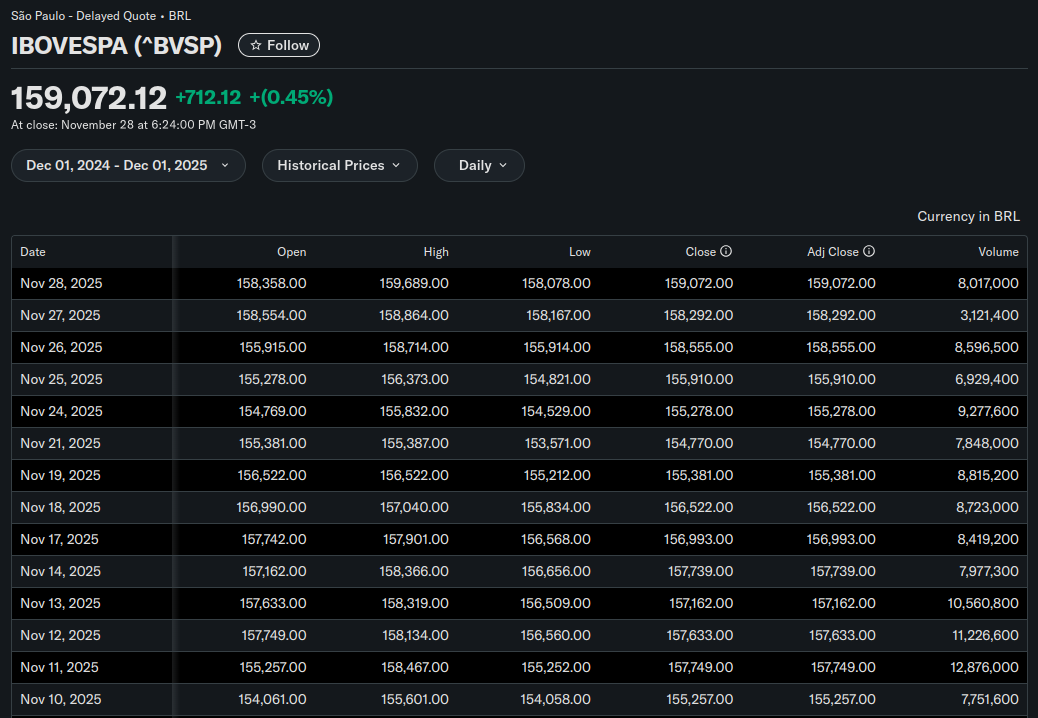
\includegraphics[width=0.8\textwidth]{figuras/indices.png}
%     \caption{Índices diários do IBOVESPA. \footcite{site10} }
%     \label{fig:indices}
% \end{figure}

% \end{frame}


% \begin{frame}{Modelos de Previsão}
% \begin{itemize}
%     \item ML clássico: SVR, CART, MLP.
%     \item \textit{Deep Learning}: LSTM para dependências de longo prazo em séries financeiras.
%     \item \textit{Ensembles}: \textit{Bagging/Boosting}.
% \end{itemize}
% \end{frame}

% \begin{frame}{Modelos de Previsão}
% \begin{figure}[H]
%     \centering
%     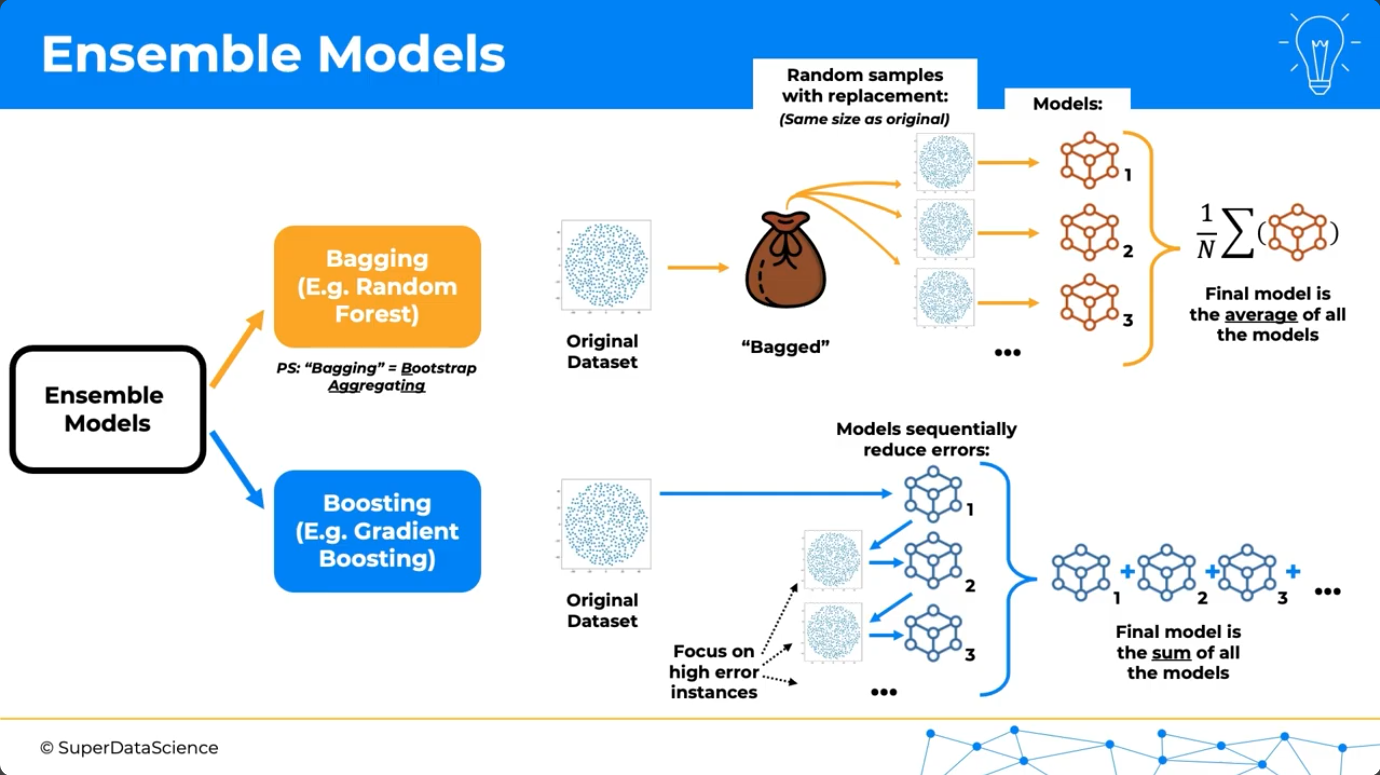
\includegraphics[width=0.8\textwidth]{figuras/ensembles.png}
%     \caption{Diferença entre \textit{ensembles} de redes neurais e \textit{ensembles} de árvores de decisão (Fonte: \footcite{site11})}
%     \label{fig:ensembles}
% \end{figure}
% \end{frame}

% \begin{frame}{Modelos de Previsão}
% \footnotesize
% \setlength{\tabcolsep}{3pt}
% \renewcommand{\arraystretch}{1.1}
% \begin{table}
% \centering
% \caption{Escolha e Análise dos Modelos de Previsão}
% \begin{tabular}{|>{\raggedright\arraybackslash}p{2.8cm}|>{\raggedright\arraybackslash}p{6.8cm}|}
% \hline
% \textbf{Artigo} & \textbf{Modelo Escolhido} \\
% \hline
% Giacomel (2016) & \textit{Ensembles} de Redes Neurais MLP \\ 
% \hline
% Dametto (2018) & \textit{Ensemble} de Redes Neurais MLP, NARX, LSTM \\ 
% \hline
% Ferro et al. (2024) & \textit{Ensembles} dos métodos MLP, SVR, CART, ARIMA \\ 
% \hline
% Nelson (2017) & Rede Neural LSTM \\ 
% \hline
% Ayatollahi e Jafari (2025) & \textit{Ensemble} de Árvores de Decisão (\textit{XGBoost}) \\ 
% \hline
% Benhamou et al. (2021) & GBDT (\textit{Gradient Boosting Decision Trees}) \\ 
% \hline
% Gupta et al. (2025) & Rede Neural LSTM \\ 
% \hline
% Gil et al. (2024) & xLSTM-TS (Extended LSTM) \\ 
% \hline
% Hertel et al. (2025) & Transformer \\ 
% \hline
% \end{tabular}
% \end{table}
% \end{frame}

% \begin{frame}{Objetivos de Previsão}
% \begin{itemize}
%     \item Regressão: prever valor futuro do índice/preço
%     \begin{itemize}\setlength\itemsep{2pt}
%         \item métricas de erro (MSE, RMSE, MAPE) e ajuste ($R^2$).
%     \end{itemize}
%     \item Classificação: direção de movimento (alta/baixa) ou detecção de crises (\textit{crashes}).
%     \begin{itemize}\setlength\itemsep{2pt}
%         \item métricas de classificação: Acurácia;
%         \item cenários desbalanceados, usar Precisão, \textit{Recall}, \textit{F1-Score}.
%     \end{itemize}
% \end{itemize}
% \end{frame}

% \begin{frame}{Fontes de Dados}
% \begin{itemize}
%     \item Mercados:
%     \begin{itemize}\setlength\itemsep{2pt}
%         \item Desenvolvidos (S\&P 500) têm menor volatilidade
%         \item Emergentes (IBOVESPA, TEPIX, HDFC) são mais instáveis e desafiadores.
%     \end{itemize}
%     \item \textit{Features}: OHLCV, indicadores técnicos e variáveis exógenas (ex.: câmbio).
%     \item Granularidade e período
% \end{itemize}
% \end{frame}

% \begin{frame}{Fontes de Dados}
% \begin{figure}[H]
%     \centering
%     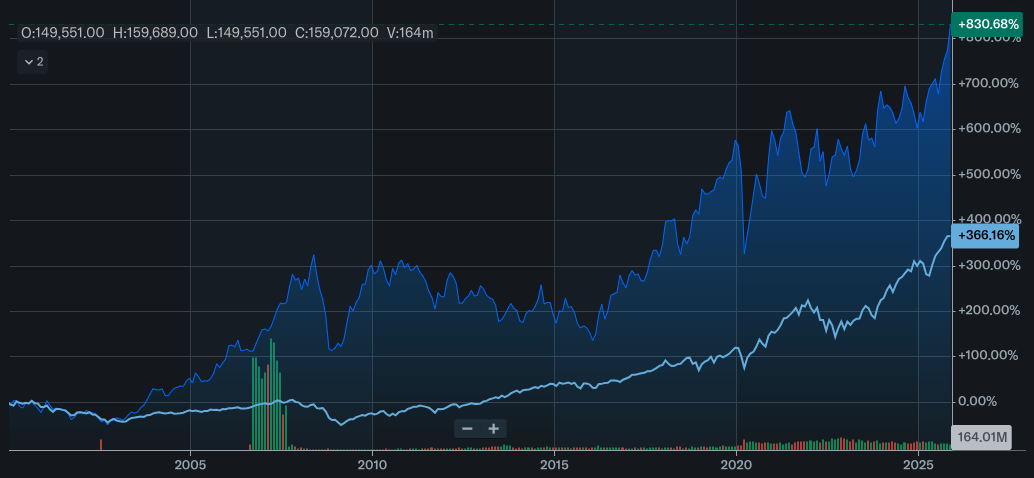
\includegraphics[width=0.9\textwidth]{figuras/mercados.png}
%     \caption{Volatilidade entre os mercados IBOVESPA (azul escuro) e S\&P 500 (azul claro) desde 2000 (Fonte: \footcite{site12})}
%     \label{fig:bolsas}
% \end{figure}
% \end{frame}

% \begin{frame}{Resumo dos Artigos}
% \footnotesize
% \setlength{\tabcolsep}{2.5pt}
% \renewcommand{\arraystretch}{1.1}
% \begin{table}
% \centering
% \caption{Objetivo de previsão e dados utilizados na literatura}
% \begin{tabular}{|>{\raggedright\arraybackslash}p{2.4cm}|>{\raggedright\arraybackslash}p{3.4cm}|>{\raggedright\arraybackslash}p{3.4cm}|}
% \hline
% \textbf{Artigo} & \textbf{Objetivo de Previsão} & \textbf{Dados Utilizados} \\
% \hline
% Giacomel (2016) & Classificação de movimento: alta/baixa & Ações mais negociadas dos mercados S\&P 500 e BOVESPA \\
% \hline
% Dametto (2018) & Regressão & IBOVESPA e cotação do Dólar \\
% \hline
% Ferro et al. (2024) & Regressão & IBOVESPA e S\&P 500 \\
% \hline
% Nelson (2017) & Classificação de movimento: alta/baixa & Ativos de maior negociação do IBOVESPA \\
% \hline
% Ayatollahi e Jafari (2025) & Classificação de risco: \textit{crash event} & TEPIX \\
% \hline
% Benhamou et al. (2021) & Classificação de risco: regime de crise/normal & S\&P 500 \\
% \hline
% Gupta et al. (2025) & Regressão & Ação HDFC \textit{Bank} \\
% \hline
% Gil et al. (2024) & Regressão e Classificação Direcional & S\&P 500 e EWZ \\
% \hline
% Hertel et al. (2025) & Regressão & Séries temporais públicas \\
% \hline
% \end{tabular}
% \end{table}
% \end{frame}

% \begin{frame}{Frameworks e Ferramentas}
% \begin{itemize}
%     \item \textbf{\textit{Deep Learning}}: \textit{Keras}/\textit{TensorFlow} para redes recorrentes.
%     \item \textbf{ML Clássico e \textit{Ensembles}}: \textit{Scikit-learn} biblioteca de aprendizado de máquina de fácil implementação.
%     \item \textbf{\textit{Boosting} e Árvores}: \textit{LightGBM} e \textit{XGBoost}, otimizados para algoritmo GBDT.
% \end{itemize}
% \end{frame}

% \begin{frame}{xAI: SHAP}
% \begin{itemize}
%     \item Desafio de entender como e por que um modelo chegou a um resultado específico.
%     \item SHAP: explica a contribuição de cada variável para a previsão final.
%     \item Crises e risco: SHAP em GBDT para identificar variáveis mais importantes \footcite{Benhamou2021XAIPlanning}.
%     \item LSTM + SHAP: explica contribuição temporal de cada \textit{time-step} na previsão de preço \footcite{Gupta2025Interpretable}.
% \end{itemize}
% \end{frame}

%-------------------------------------------------------
\section{Metodologia}
%-------------------------------------------------------
\begin{frame}{Escopo do Projeto}
\begin{columns}
    \begin{column}{0.4\textwidth}
        \centering
        \vspace{0.3\textheight}
        Figura: Fluxo de Projeto
        \label{fig:fluxo_processamento}
    \end{column}
    \begin{column}{0.6\textwidth}
    \end{column}
\end{columns}

\begin{textblock*}{12cm}(6.7cm,0.2cm)
    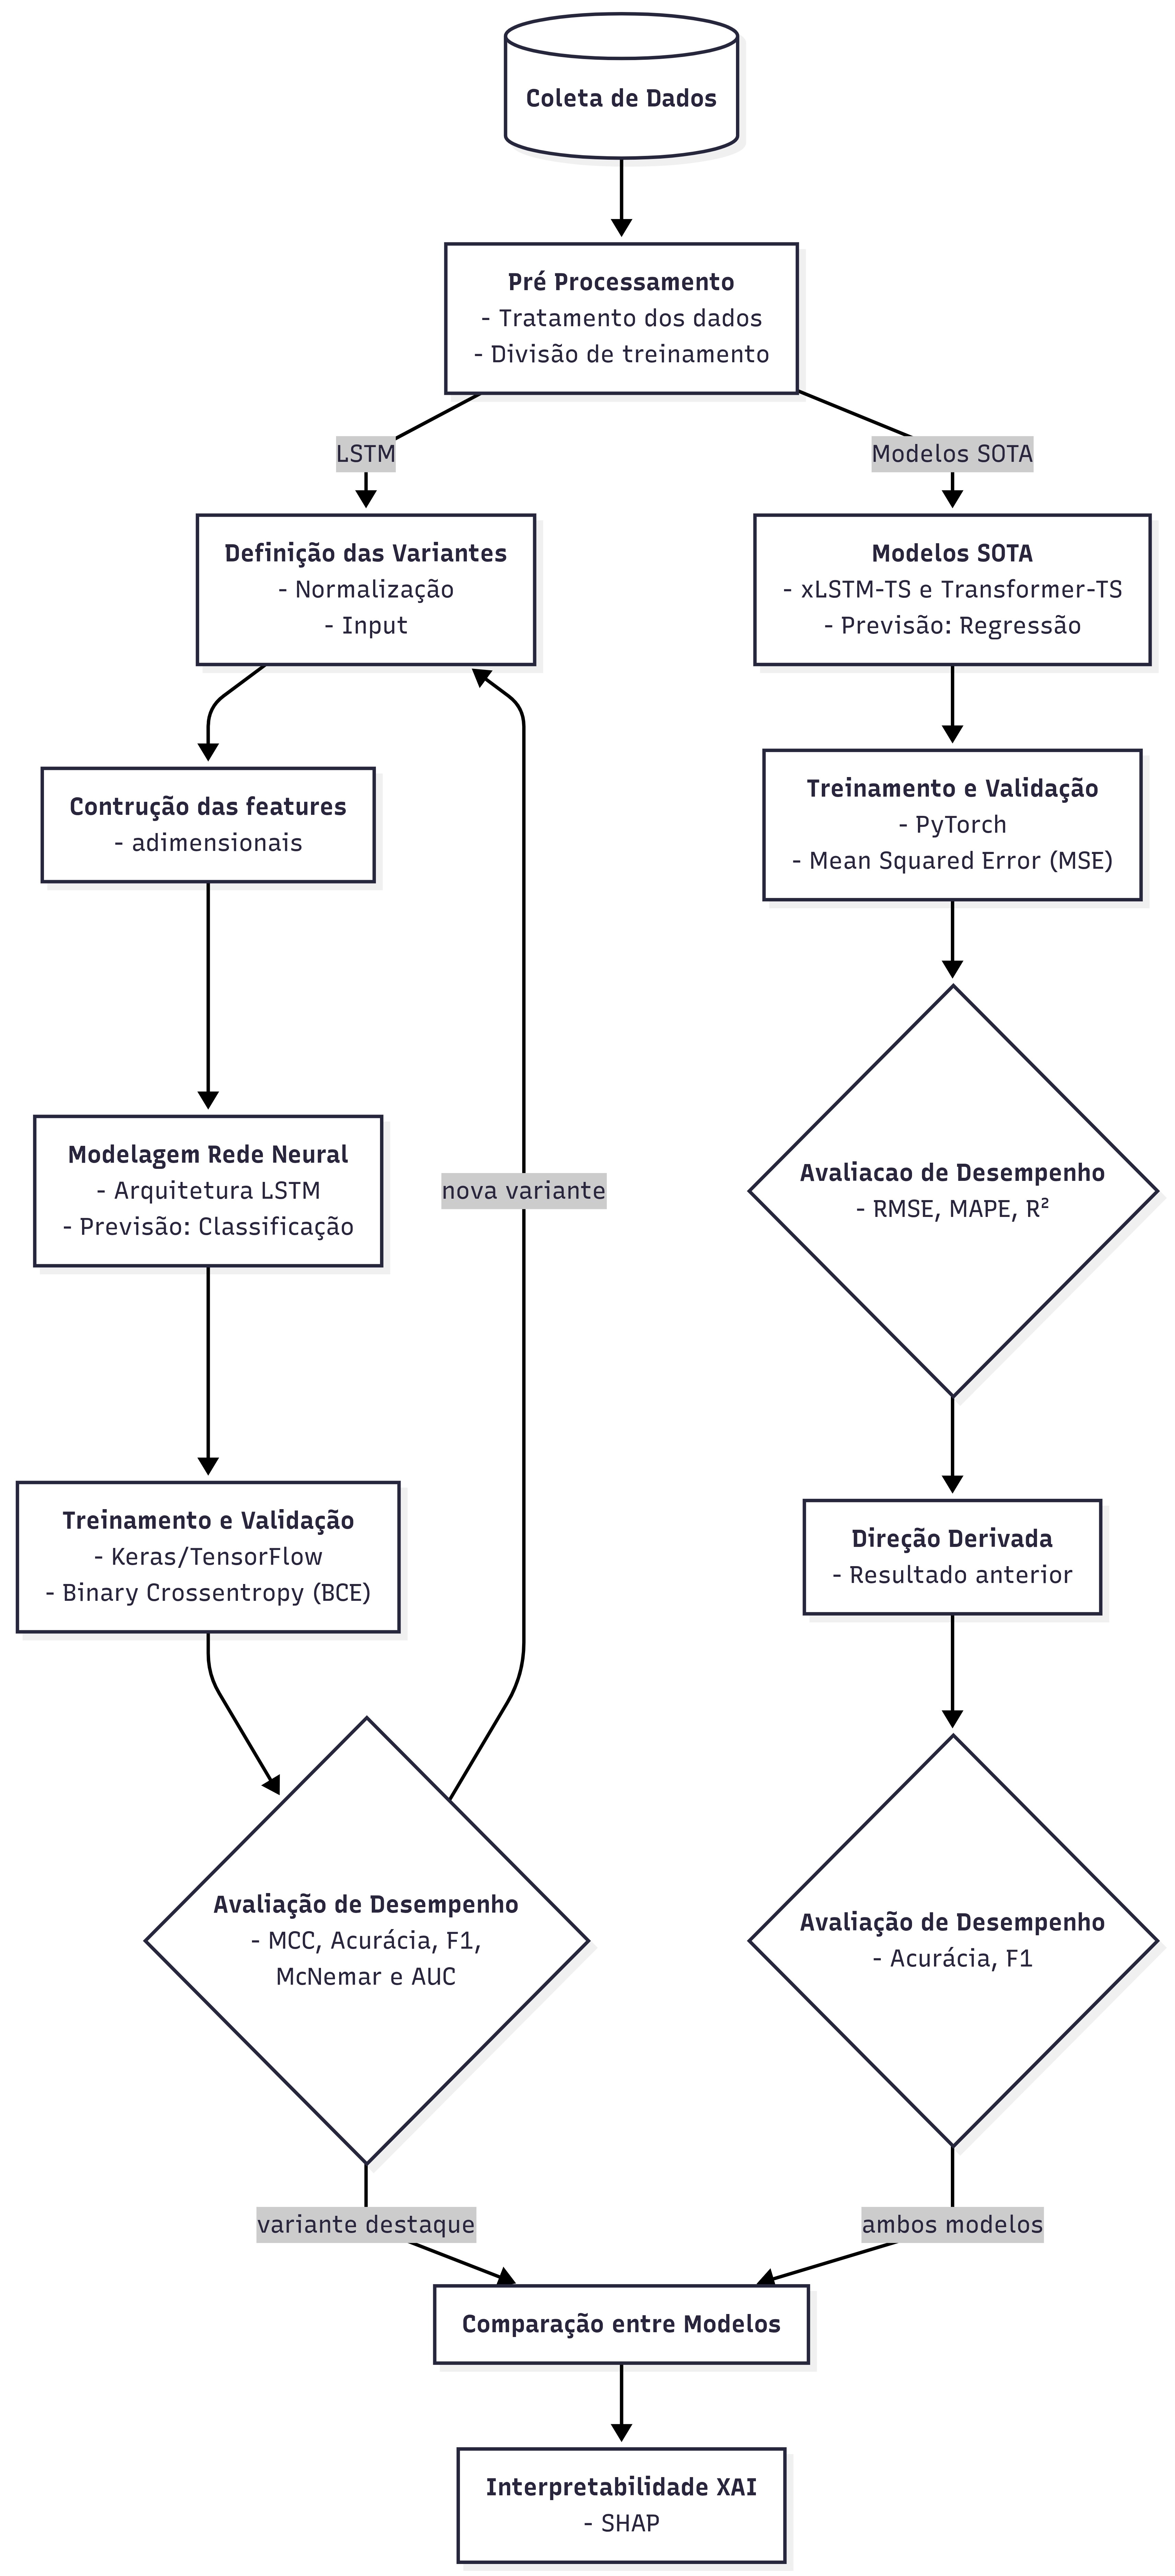
\includegraphics[height=0.97\textheight]{figuras/flow.png}
\end{textblock*}
\end{frame}

\begin{frame}{Escopo do Projeto}
\begin{enumerate}
    \item \textbf{Aquisição de Dados e Pré-processamento:} Coleta de preços históricos e tratamento.
    \item \textbf{\textit{Ablation Study} (LSTM \textit{baseline}):} Construção de \textit{features} e teste de variantes.
    \item \textbf{Modelos \textit{SOTA}:} Previsões com os modelos \textit{SOTA}: xLSTM-TS e Transformer-TS.
    \item \textbf{Comparação de Desempenho dos Modelos:} Avaliação dos modelos de acordo com as métricas de classificação.
    \item \textbf{Interpretabilidade xAI:} Aplicação do SHAP para identificar a importância de cada \textit{timestep}.
\end{enumerate}
\end{frame}

\begin{frame}{Aquisição de Dados}
\textbf{Fonte e Período:}
\begin{itemize}
    \item S\&P 500 diário: 03/01/2000 a 30/12/2024
    \item Variáveis OHLCV (\textit{Open}, \textit{High}, \textit{Low}, \textit{Close}, \textit{Volume})
\end{itemize}

\vspace{0.3cm}
\textbf{Divisão Temporal:}
\begin{itemize}
    \item 84\% treino (2000--2020): 5.282 dias
    \item 8\% validação (2021--2022): 503 dias
    \item 8\% teste (2023--2024): 503 dias
\end{itemize}

\vspace{0.3cm}
\textbf{Tratamento de Ruído:}
\begin{itemize}
    \item Sem dados faltante e volume zero imputado pela mediana móvel
\end{itemize}
\end{frame}

\begin{frame}{Engenharia de Features}
\textbf{18 Features em 4 Categorias:}
\begin{itemize}
    \item \textbf{\textit{Log-retornos} e defasagens (7 \textit{features})}
    \item \textbf{Tendência relativa (3 \textit{features})}
    \item \textbf{Volatilidade realizada (2 \textit{features})}
    \item \textbf{Volume e amplitude (6 \textit{features})}
\end{itemize}
\end{frame}

\begin{frame}{Variantes do Ablation Study}
\footnotesize
\setlength{\tabcolsep}{2pt}
\renewcommand{\arraystretch}{1.0}
\begin{table}
\centering
\caption{Variantes do Ablation Study de Pré-processamento}
\begin{tabular}{|c|c|c|p{0.5\textwidth}|}
\hline
\textbf{Variante} & \textbf{Input} & \textbf{Normalização} & \textbf{Motivação} \\
\hline
A & \textit{Close} bruto & \textit{Z-score} & \textit{Baseline} padrão da literatura. Ponto de referência mínimo. \\
\hline
B & \textit{Close} \textit{DWT} & \textit{Z-score} & Aplica \textit{DWT} antes de calcular as 18 \textit{features}. Avalia se remover ruído melhora a aprendizagem. \\
\hline
C & \textit{Log-retornos} & \textit{Z-score} & Substitui \textit{Close} pelo \textit{log-retorno} diário. Avalia previsão em série estacionária. \\
\hline
D & \textit{Log-ret.} \textit{DWT} & \textit{Z-score} & Aplica \textit{DWT} nos \textit{log-returns}. Combina estacionarização com \textit{DWT}. \\
\hline
E & \textit{Close} bruto & \textit{Min-Max} & Normalização em intervalo [0,1]. Testa sensibilidade a valores extremos do treino. \\
\hline
F & \textit{Close} \textit{DWT} & \textit{Min-Max} & Combina \textit{DWT} com normalização \textit{Min-Max}. \\
\hline
\end{tabular}
\end{table}
\end{frame}

\begin{frame}{Arquiteturas dos Modelos}
\textbf{LSTM:}
\begin{itemize}
    \item Classificação Binária Direta - P(sobe) = [0,1]
    \item \textit{Framework}: \textit{Keras}/\textit{TensorFlow} 2.15
    \item \textit{Early stopping}: paciência 10 épocas
\end{itemize}
\end{frame}

\begin{frame}{Arquiteturas dos Modelos}
\textbf{xLSTM-TS:}
\begin{itemize}
    \item Regressão com Direção Derivada
    \begin{itemize}
        \item Para cada dia $t$, prever se o preço de $t+1$ será maior (classe 1) ou menor (classe 0)
    \end{itemize}
    \item \textit{Framework}: \textit{PyTorch} 2.3.1
    \item \textit{Early stopping}: paciência 40 épocas
    \item Pré-processamento: \textit{DWT} \textit{causal} + \textit{Min-Max}
\end{itemize}

\vspace{0.3cm}
\textbf{Transformer-TS (Regressão com Direção Derivada):}
\begin{itemize}
    \item Regressão com Direção Derivada
    \begin{itemize}
        \item Para cada dia $t$, prever se o preço de $t+1$ será maior (classe 1) ou menor (classe 0)
    \end{itemize}
    \item \textit{Framework}: \textit{PyTorch} 2.3.1
    \item \textit{Early stopping}: paciência 40 épocas
    \item Pré-processamento: \textit{DWT} \textit{causal} + \textit{Min-Max}
\end{itemize}
\end{frame}

\begin{frame}{Métricas de Avaliação}

\vspace{0.3cm}
\textbf{Métricas de Classificação:}
\begin{itemize}
    \item \textit{MCC}: considera desequilíbrio de classes
    \item Acurácia, \textit{F1-Score} e \textit{AUC-ROC}: taxas de acerto
\end{itemize}

\vspace{0.3cm}
\textbf{Métricas de Regressão (Modelos SOTA):}
\begin{itemize}
    \item \textit{RMSE}, \textit{MAPE} e $R^2$
\end{itemize}

\vspace{0.3cm}
\textbf{Teste de \textit{McNemar}:}
\begin{itemize}
    \item Verifica significância estatística
\end{itemize}
\end{frame}

\begin{frame}{Estratégia de Interpretabilidade (xAI)}
\textbf{Aplicação do SHAP:}
\begin{itemize}
    \item Avaliação sobre 200 amostras do conjunto de teste
    \item \textit{KernelExplainer} para LSTM (modelo \textit{Keras})
    \item \textit{DeepExplainer} para modelos \textit{SOTA}
    \item Atribui a cada \textit{timestep} uma contribuição marginal para a previsão
    \item Importância global: média da magnitude $|SHAP|$ sobre todas as amostras
\end{itemize}

\vspace{0.3cm}
\textbf{Foco da Análise:}
\begin{itemize}
    \item \textbf{Contribuição Temporal:} quais períodos da memória foram mais determinantes
    \item \textbf{Concentração da Atenção:} quantos \textit{timesteps} explicam 90\% da importância total
\end{itemize}
\end{frame}

%-------------------------------------------------------
\section{Resultados}
%-------------------------------------------------------

\begin{frame}{Resultados Ablation Study}
\begin{table}
\centering
\caption{Resultados Ablation Study da LSTM}
\begin{tabular}{@{}lccccc@{}}
\toprule
\textbf{\textit{Var.}} & \textbf{\textit{Acc} Teste (\%)} & \textbf{\textit{F1} (\%)} & \textbf{\textit{MCC}} & \textbf{\textit{AUC}} & \textit{McNemar} $p$ \\
\midrule
B & \textbf{67,5} & \textbf{72,0} & \textbf{0,333} & \textbf{0,724} & $<$0,001 \\
F & 64,7 & 70,2 & 0,273 & 0,687 & 0,004 \\
D & 62,3 & 70,8 & 0,211 & 0,671 & 0,017 \\
A & 61,5 & 69,6 & 0,195 & 0,652 & 0,049 \\
C & 61,5 & 69,6 & 0,195 & 0,652 & 0,049 \\
E & 56,5 & 72,2 & 0,000 & 0,512 & 1,000 \\
\bottomrule
\end{tabular}
\end{table}
\end{frame}

\begin{frame}{Resultados Ablation Study}
\begin{figure}[H]
    \centering
    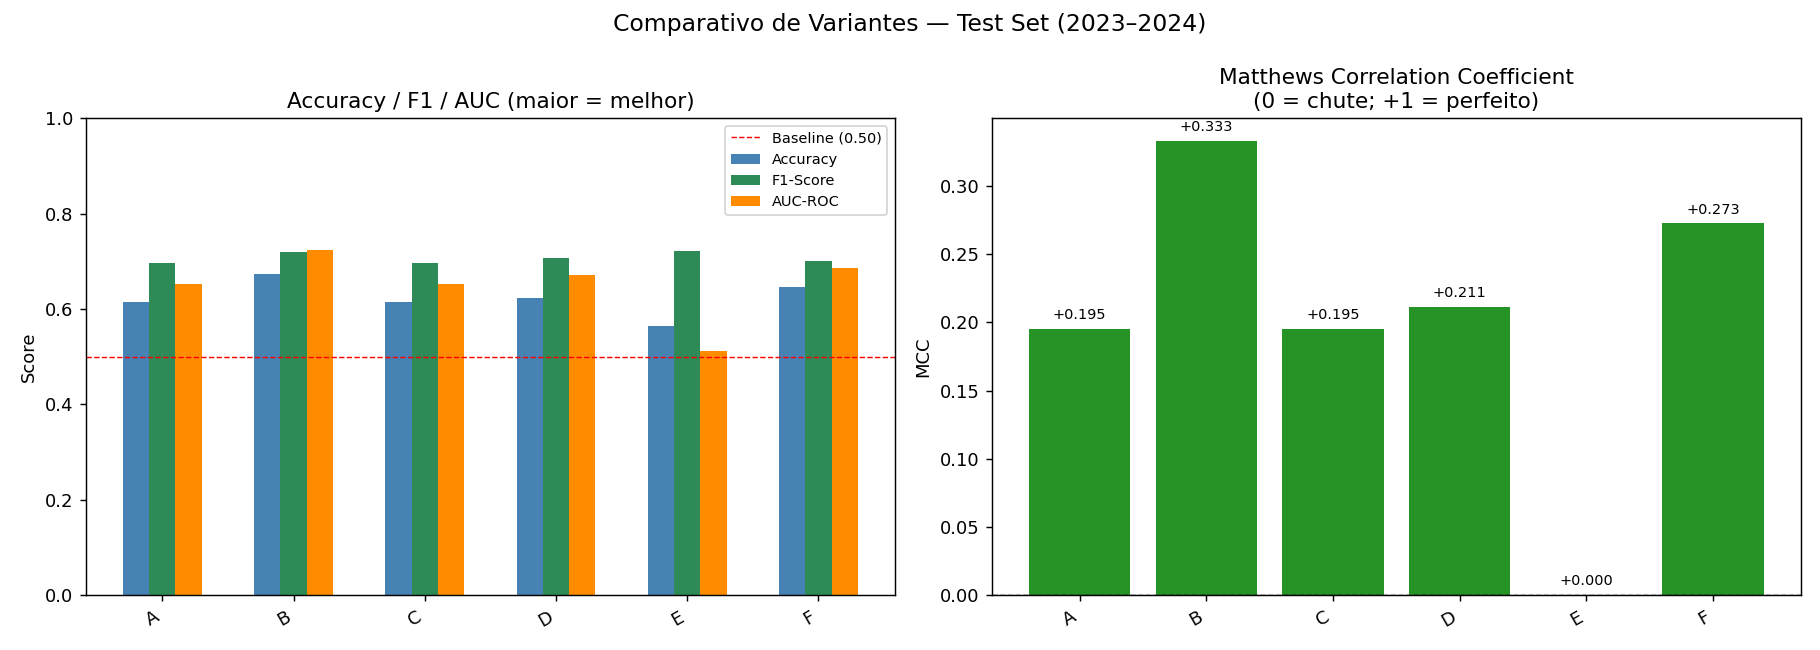
\includegraphics[width=0.9\textwidth]{figuras/comparativo_variantes.png}
    \caption{Métricas de classificação direcional no teste por variante do ablation study}
\end{figure}
\end{frame}

\begin{frame}{Resultados Ablation Study}
\begin{figure}[H]
    \centering
    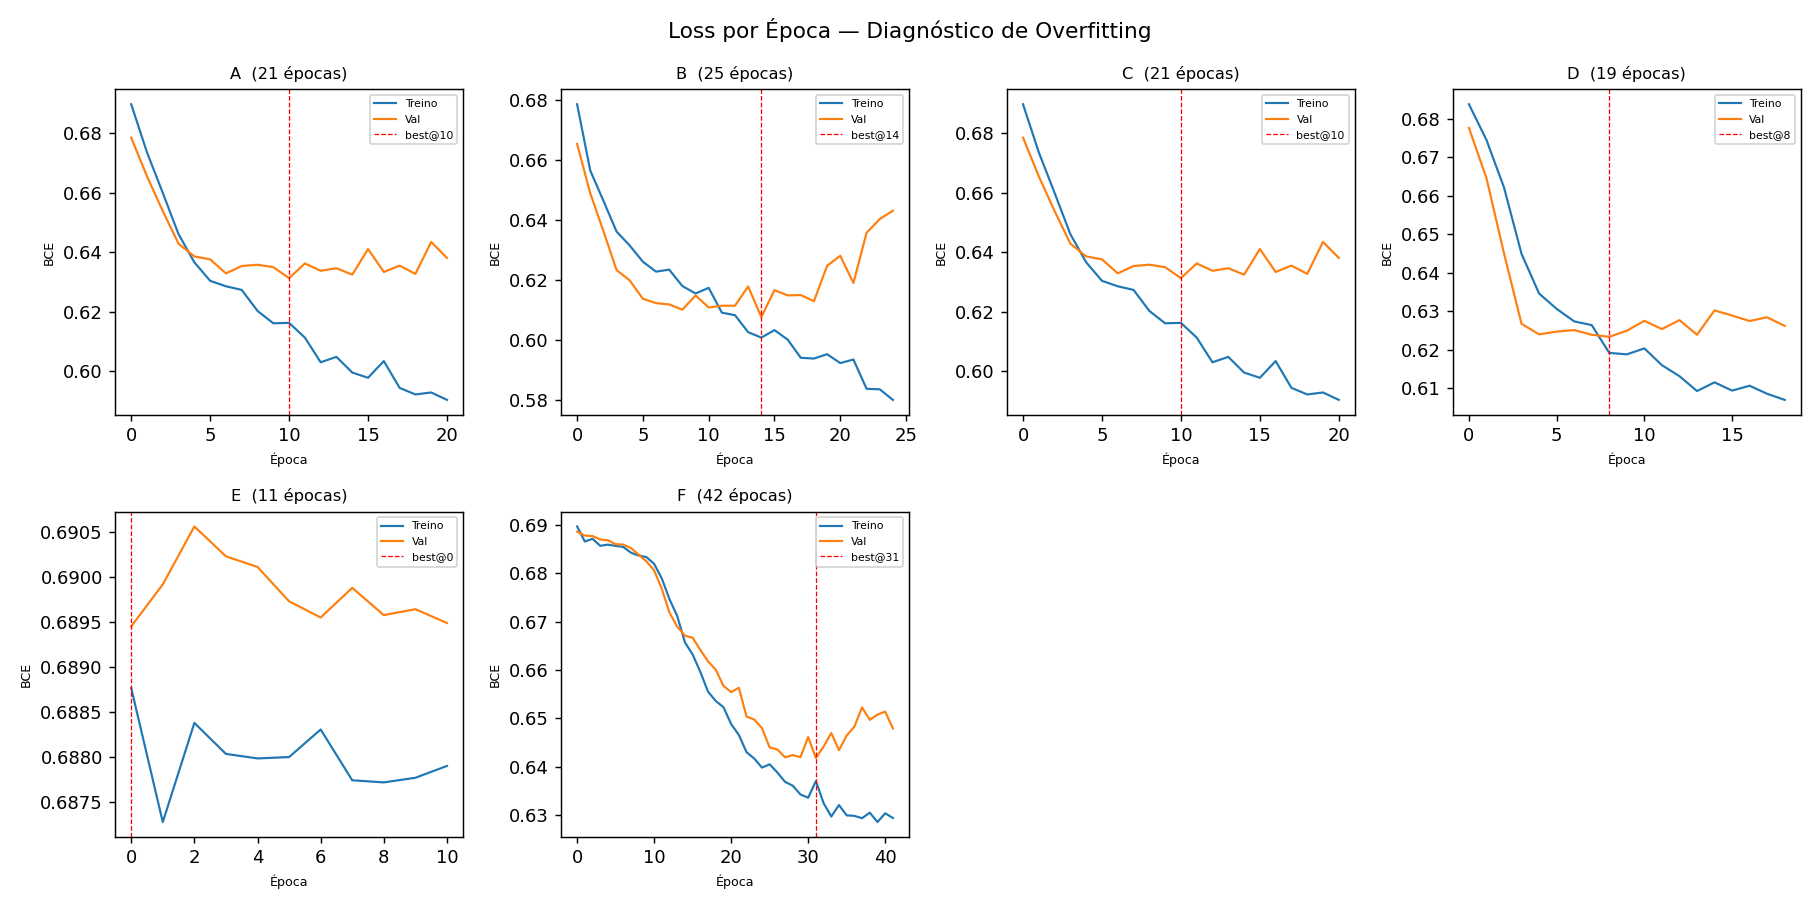
\includegraphics[width=0.9\textwidth]{figuras/overfitting_variantes.png}
    \caption{Curvas de perda de treino e validação por época para cada variante}
\end{figure}
\end{frame}

\begin{frame}{Resultados Ablation Study}
\begin{figure}[H]
    \centering
    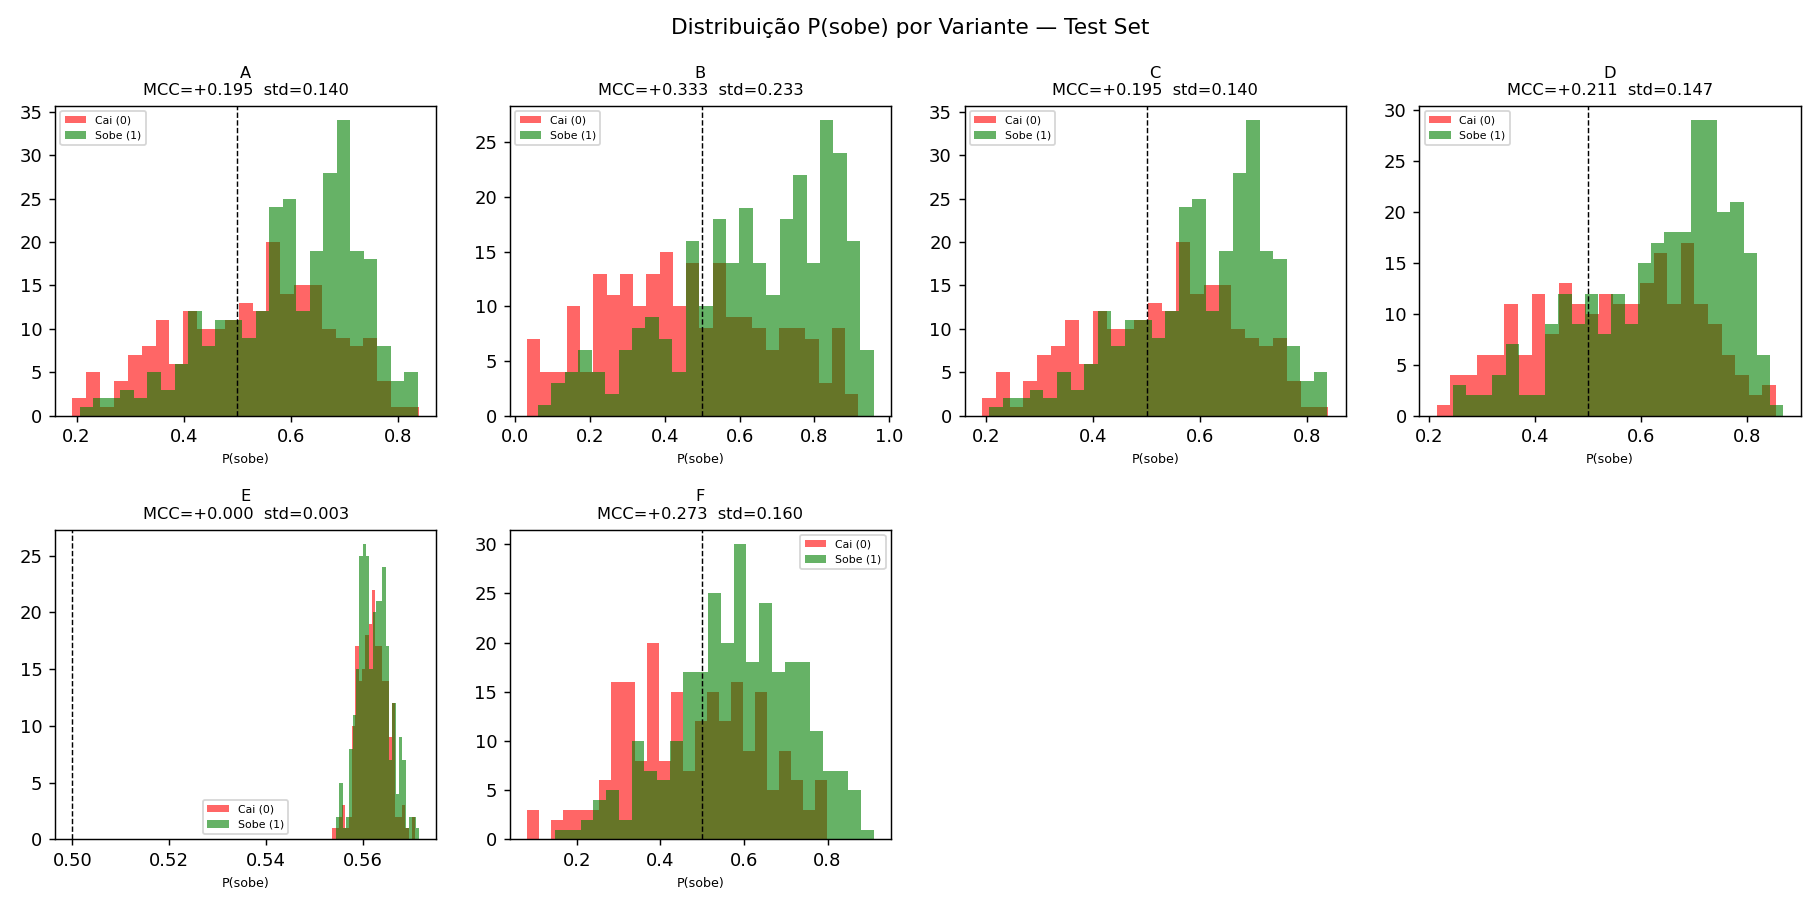
\includegraphics[width=0.9\textwidth]{figuras/probabilidades_variantes.png}
    \caption{Distribuição de $P(\textit{sobe})$ no conjunto de teste por variante e classe/valor real}
\end{figure}
\end{frame}

\begin{frame}{Desempenho Variante B}
\textbf{Variante B: \textit{Close} \textit{DWT} + \textit{Z-score}}

\vspace{0.3cm}
\begin{figure}[H]
    \centering
    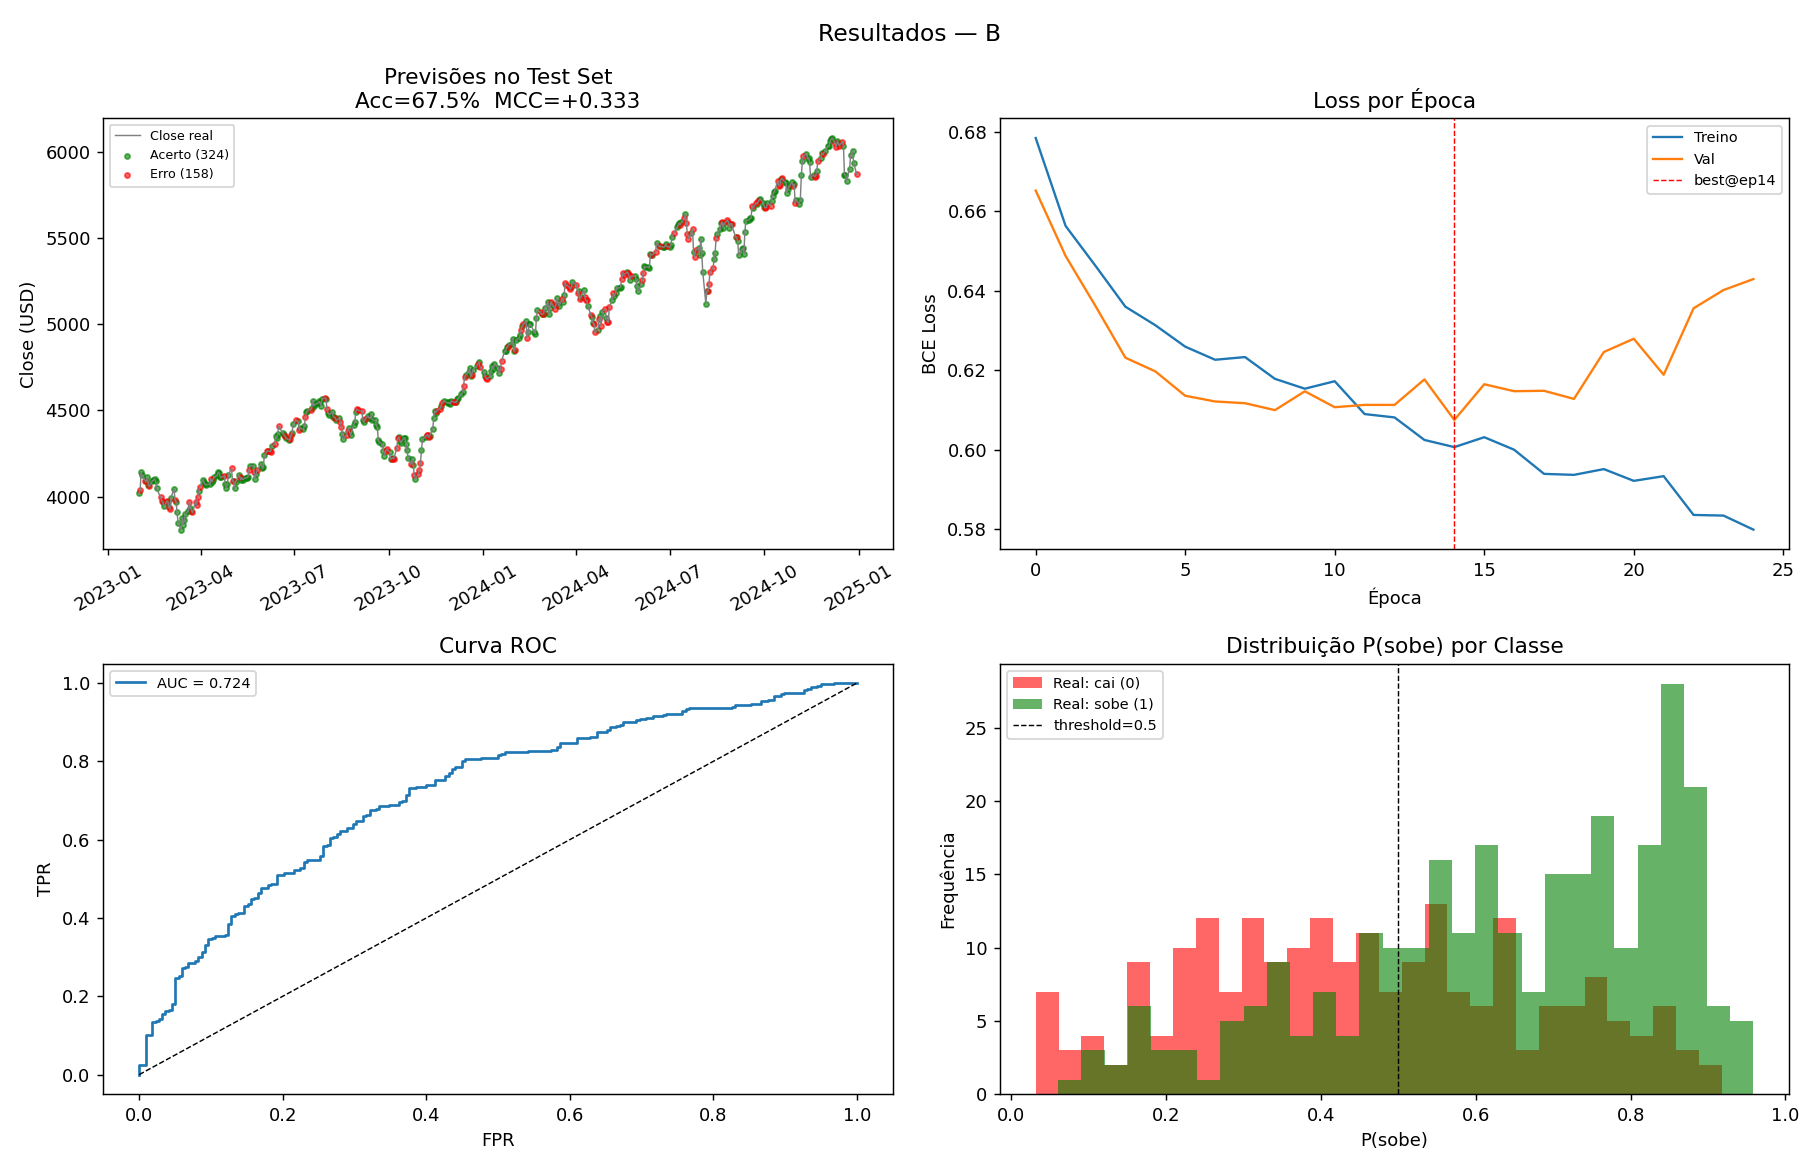
\includegraphics[width=0.8\textwidth]{figuras/resultados_B.png}
    \caption{Resultados da variante B}
\end{figure}
\end{frame}

\begin{frame}{Resultados Modelos \textit{SOTA}}
\begin{columns}
    \begin{column}{0.5\textwidth}
    \centering
    \footnotesize
    \textbf{xLSTM-TS}
    \begin{tabular}{@{}llr@{}}
    \toprule
    \textbf{\textit{Cat.}} & \textbf{Métrica} & \textbf{Valor} \\
    \midrule
    Regressão & \textit{MAE} & 235,80 USD \\
    & \textit{RMSE} & 375,40 USD \\
    & \textit{MAPE} & 4,26\% \\
    & $R^2$ & 0,662 \\
    \midrule
    Direcional & Acurácia & 75,8\% \\
    & \textit{Recall} & 76,6\% \\
    & \textit{F1} & 79,8\% \\
    \bottomrule
    \end{tabular}
    \end{column}
    \begin{column}{0.5\textwidth}
    \centering
    \footnotesize
    \textbf{Transformer-TS}
    \begin{tabular}{@{}llr@{}}
    \toprule
    \textbf{Cat.} & \textbf{Métrica} & \textbf{Valor} \\
    \midrule
    Regressão & \textit{MAE} & 541,81 USD \\
    & \textit{RMSE} & 706,64 USD \\
    & \textit{MAPE} & 10,19\% \\
    & $R^2$ & $-$0,20 \\
    \midrule
    Direcional & Acurácia & 75,6\% \\
    & \textit{Recall} & 86,9\% \\
    & \textit{F1} & 81,6\% \\
    \bottomrule
    \end{tabular}
    \end{column}
\end{columns}
\end{frame}

\begin{frame}{Resultados Visuais xLSTM-TS}
\begin{figure}[H]
    \centering
    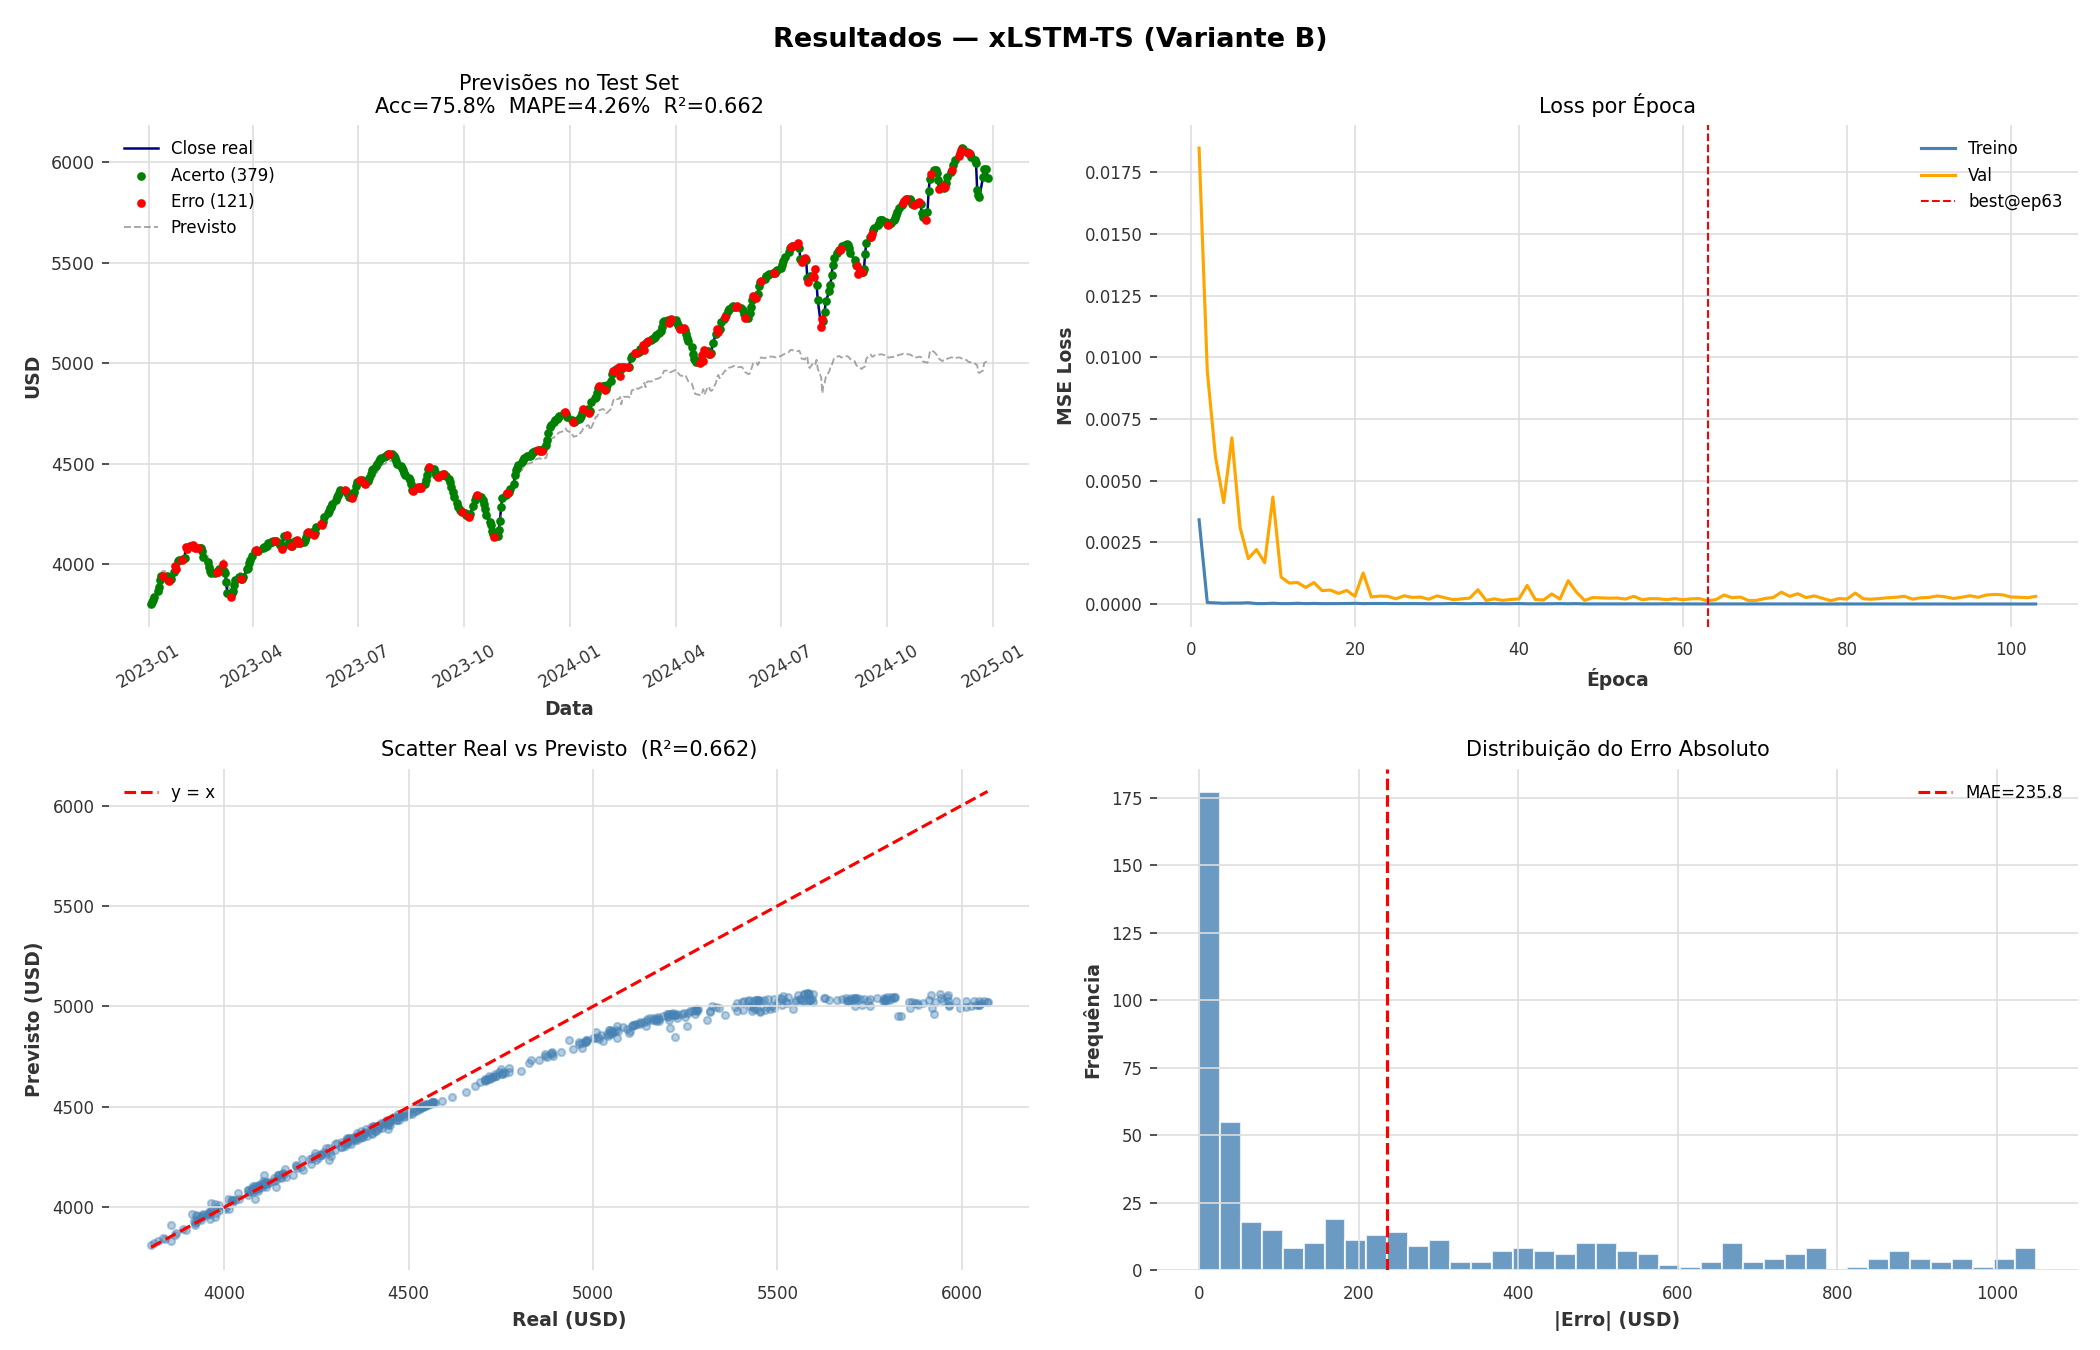
\includegraphics[width=0.9\textwidth]{figuras/xlstm_ts_resultados.png}
    \caption{Resultados do xLSTM-TS no conjunto de teste (2023--2024)}
\end{figure}
\end{frame}

\begin{frame}{Resultados Visuais Transformer-TS}
\begin{figure}[H]
    \centering
    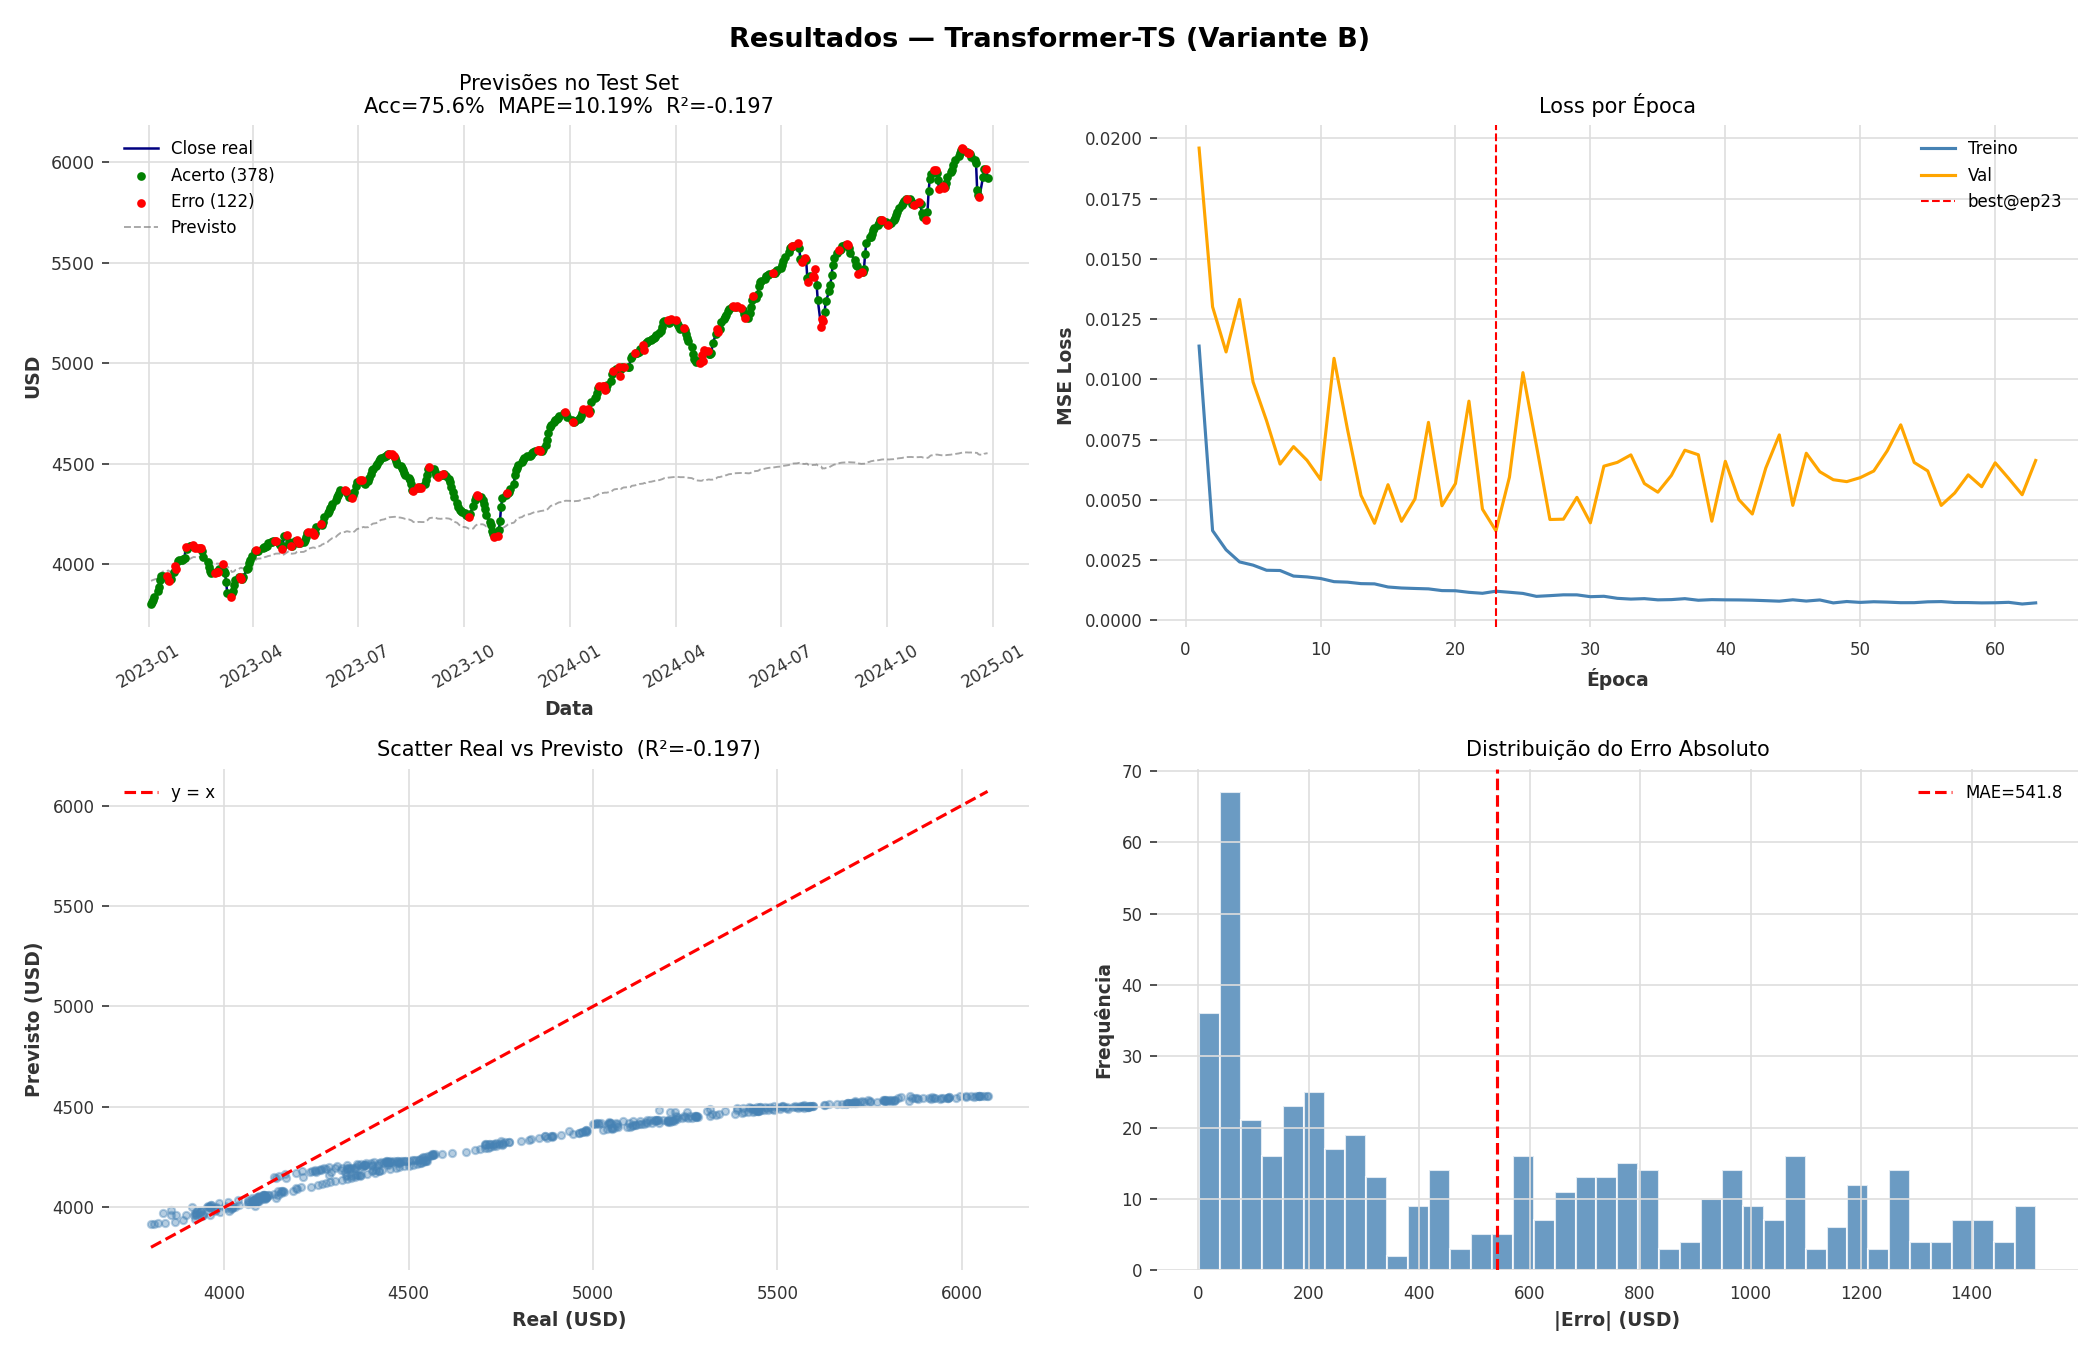
\includegraphics[width=0.9\textwidth]{figuras/transformer_ts_resultados.png}
    \caption{Resultados do Transformer-TS no conjunto de teste (2023--2024)}
\end{figure}
\end{frame}

\begin{frame}{Comparativo Desempenho Direcional}
\begin{table}
\centering
\caption{Comparativo de acurácia e F1 direcional dos três modelos no conjunto de teste}
\begin{tabular}{@{}lcc@{}}
\toprule
\textbf{Modelo} & \textbf{\textit{Acc} (\%)} & \textbf{\textit{F1} (\%)} \\
\midrule
LSTM Var.~B    & 67,5 & 72,0 \\
xLSTM-TS       & 75,8 & 79,8 \\
Transformer-TS & 75,6 & 81,6 \\
\bottomrule
\end{tabular}
\end{table}

\textbf{Observações:}
\begin{itemize}
    \item $R^2$ inferior à persistência, mas classificação direcional é superior
    \item Métricas de regressão não são adequadas para julgar viabilidade operacional
\end{itemize}
\end{frame}

\begin{frame}{Análise SHAP - LSTM}
\begin{figure}[H]
    \centering
    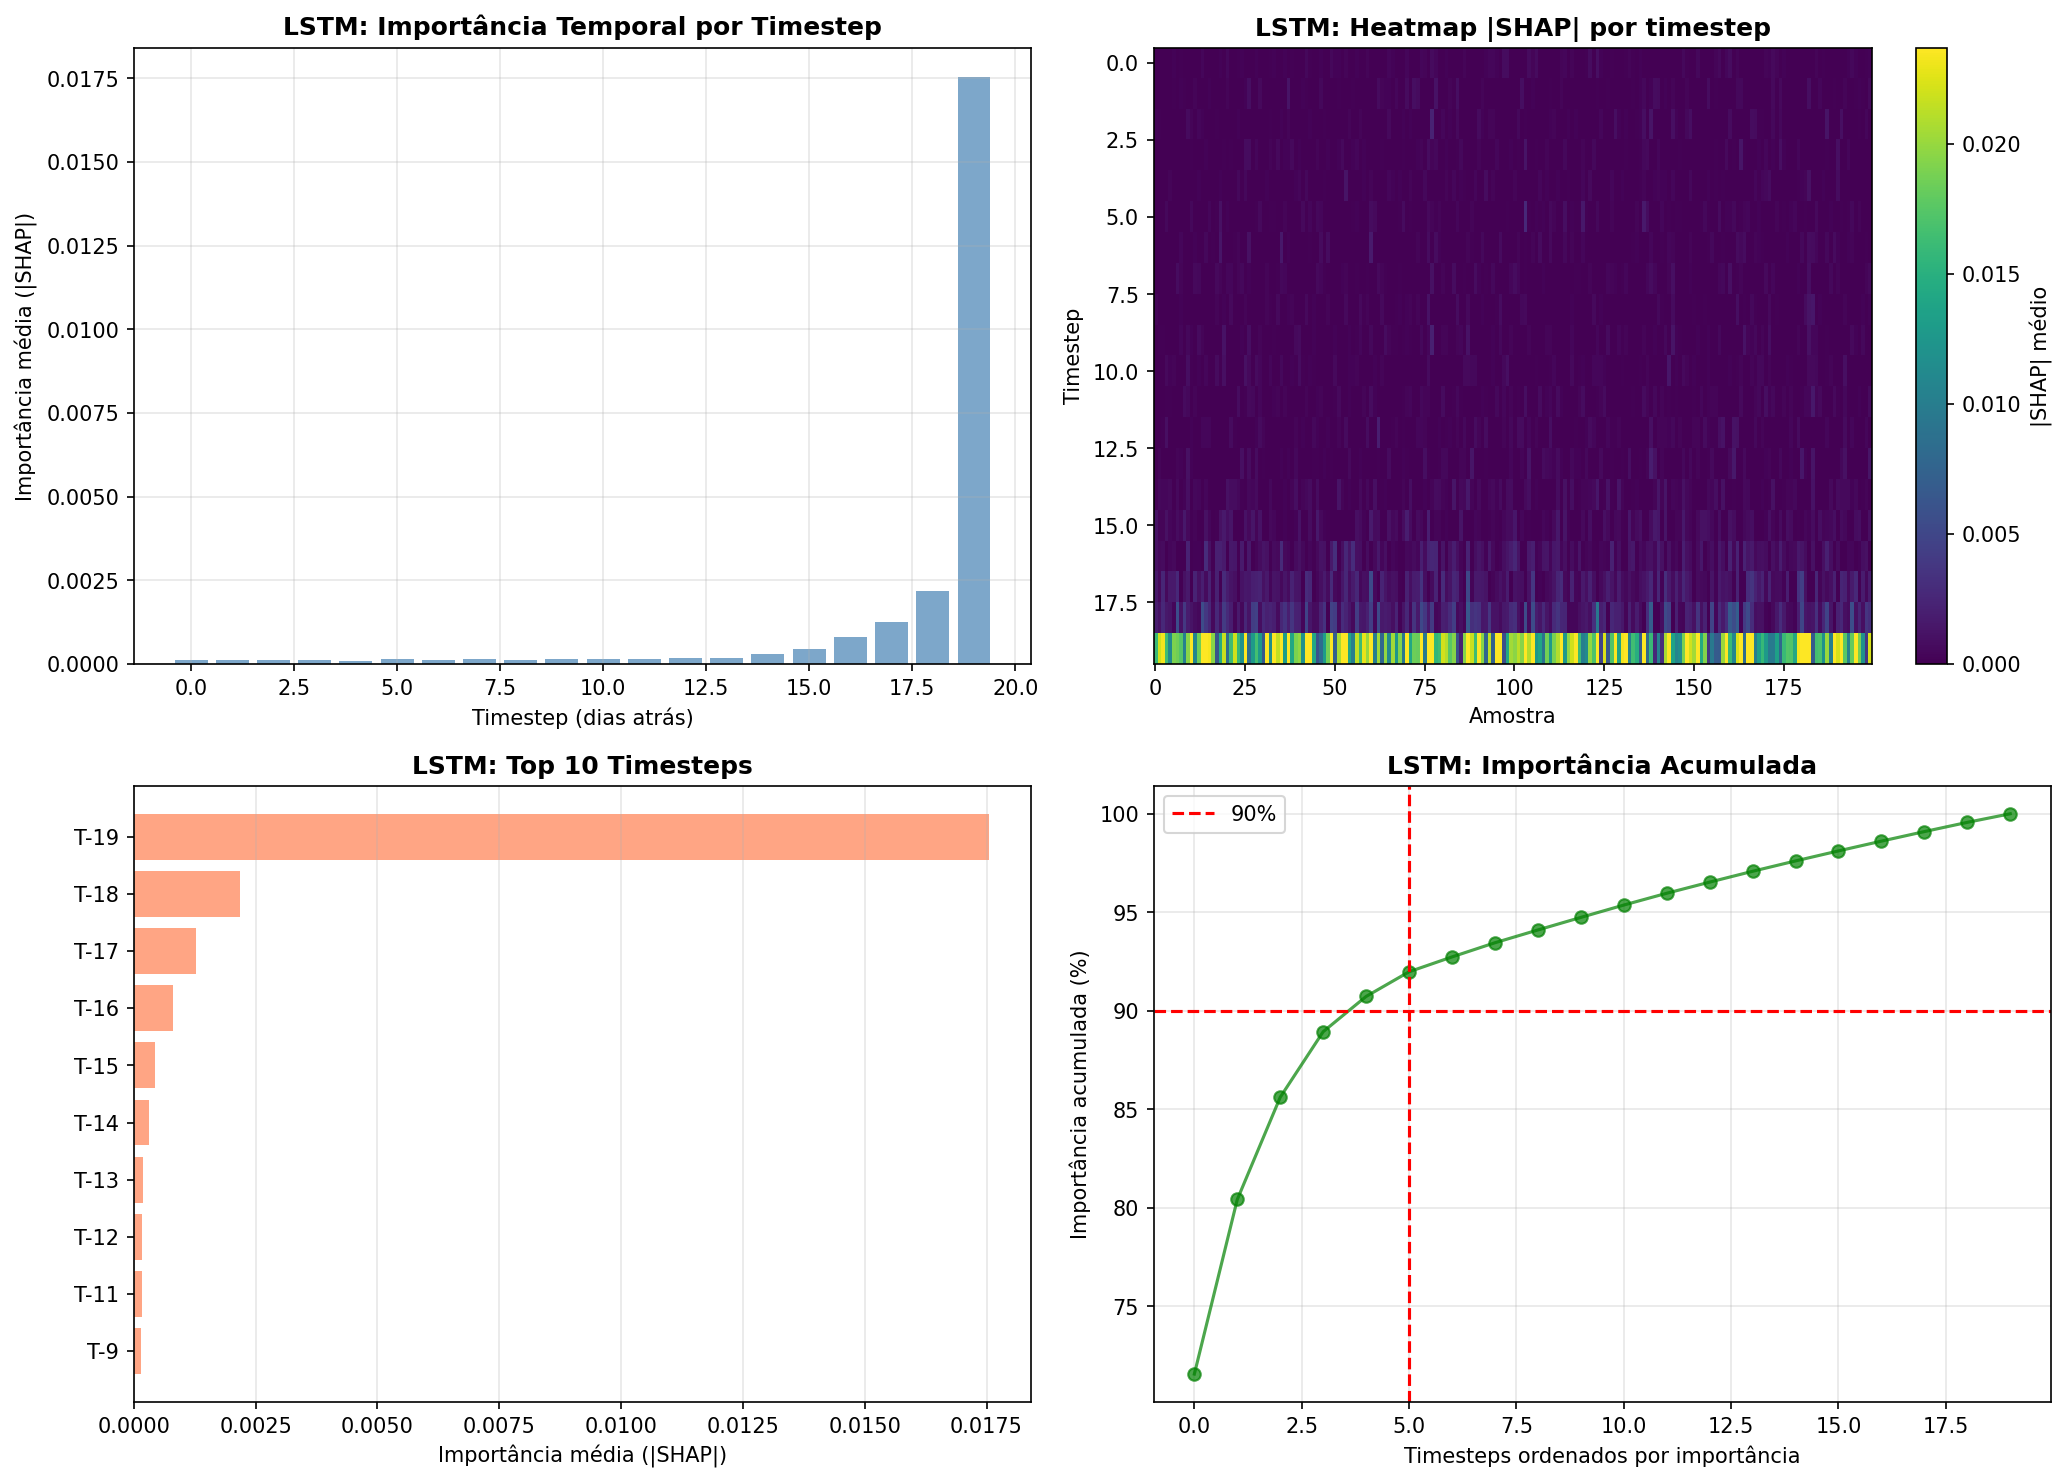
\includegraphics[width=0.85\textwidth]{figuras/shap_lstm.png}
    \caption{Análise SHAP da LSTM (Variante B) sobre 200 amostras do conjunto de teste (2023--2024)}
\end{figure}
\end{frame}

\begin{frame}{Análise SHAP - xLSTM-TS}
\begin{figure}[H]
    \centering
    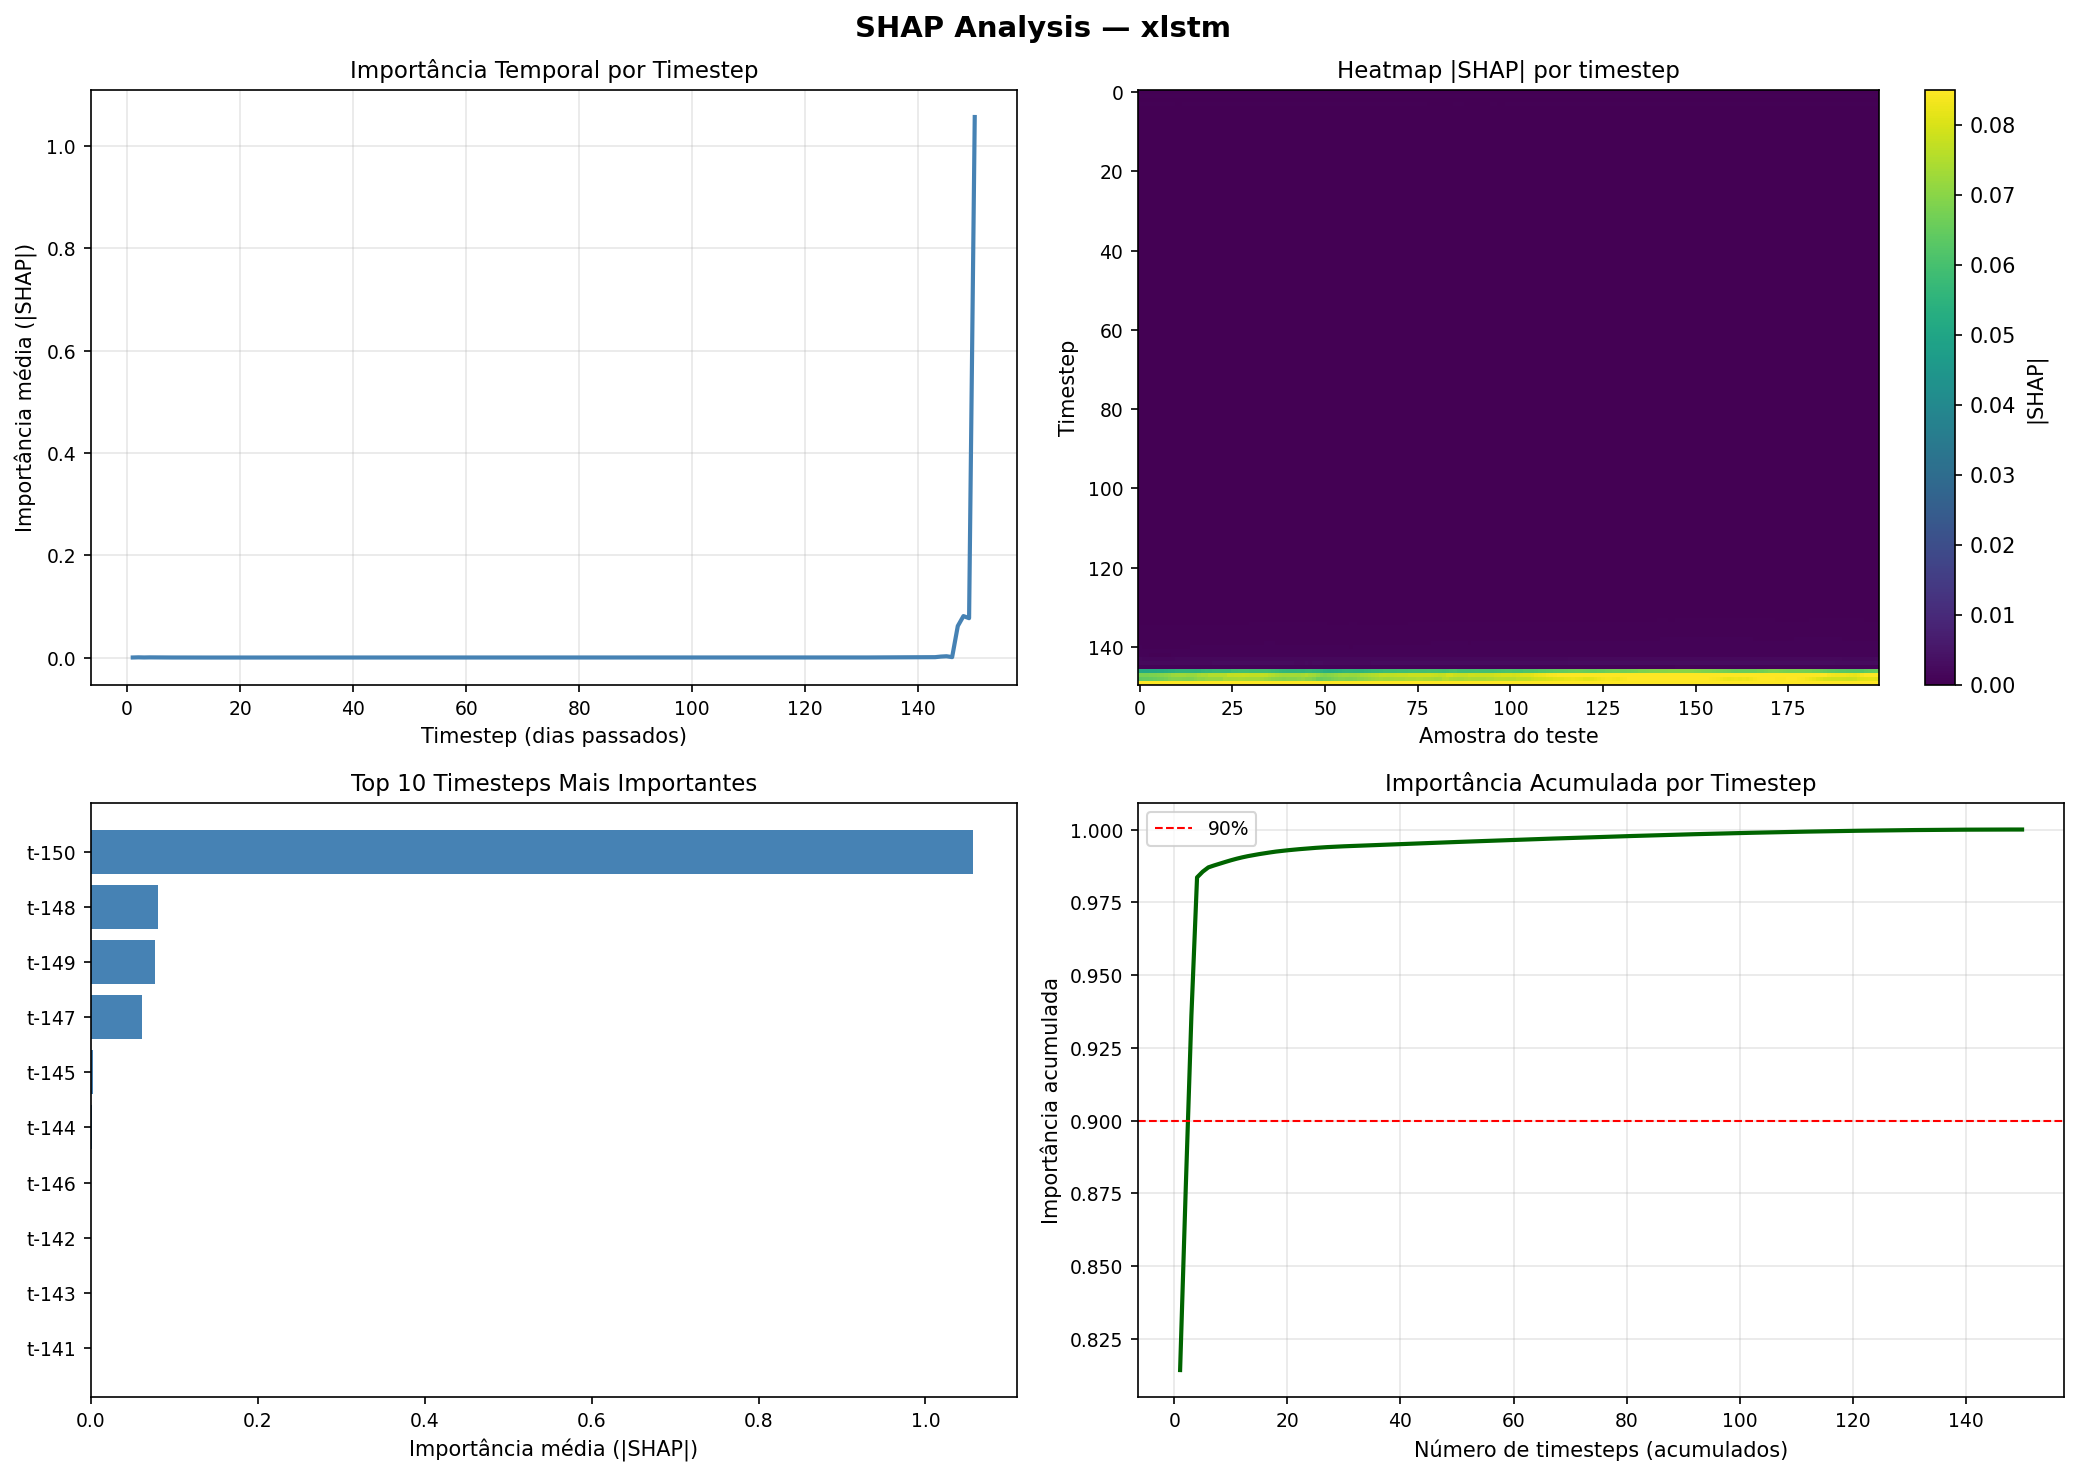
\includegraphics[width=0.85\textwidth]{figuras/shap_xlstm.png}
    \caption{Análise SHAP do xLSTM-TS no conjunto de teste (2023--2024)}
\end{figure}
\end{frame}

\begin{frame}{Análise SHAP - Transformer-TS}
\begin{figure}[H]
    \centering
    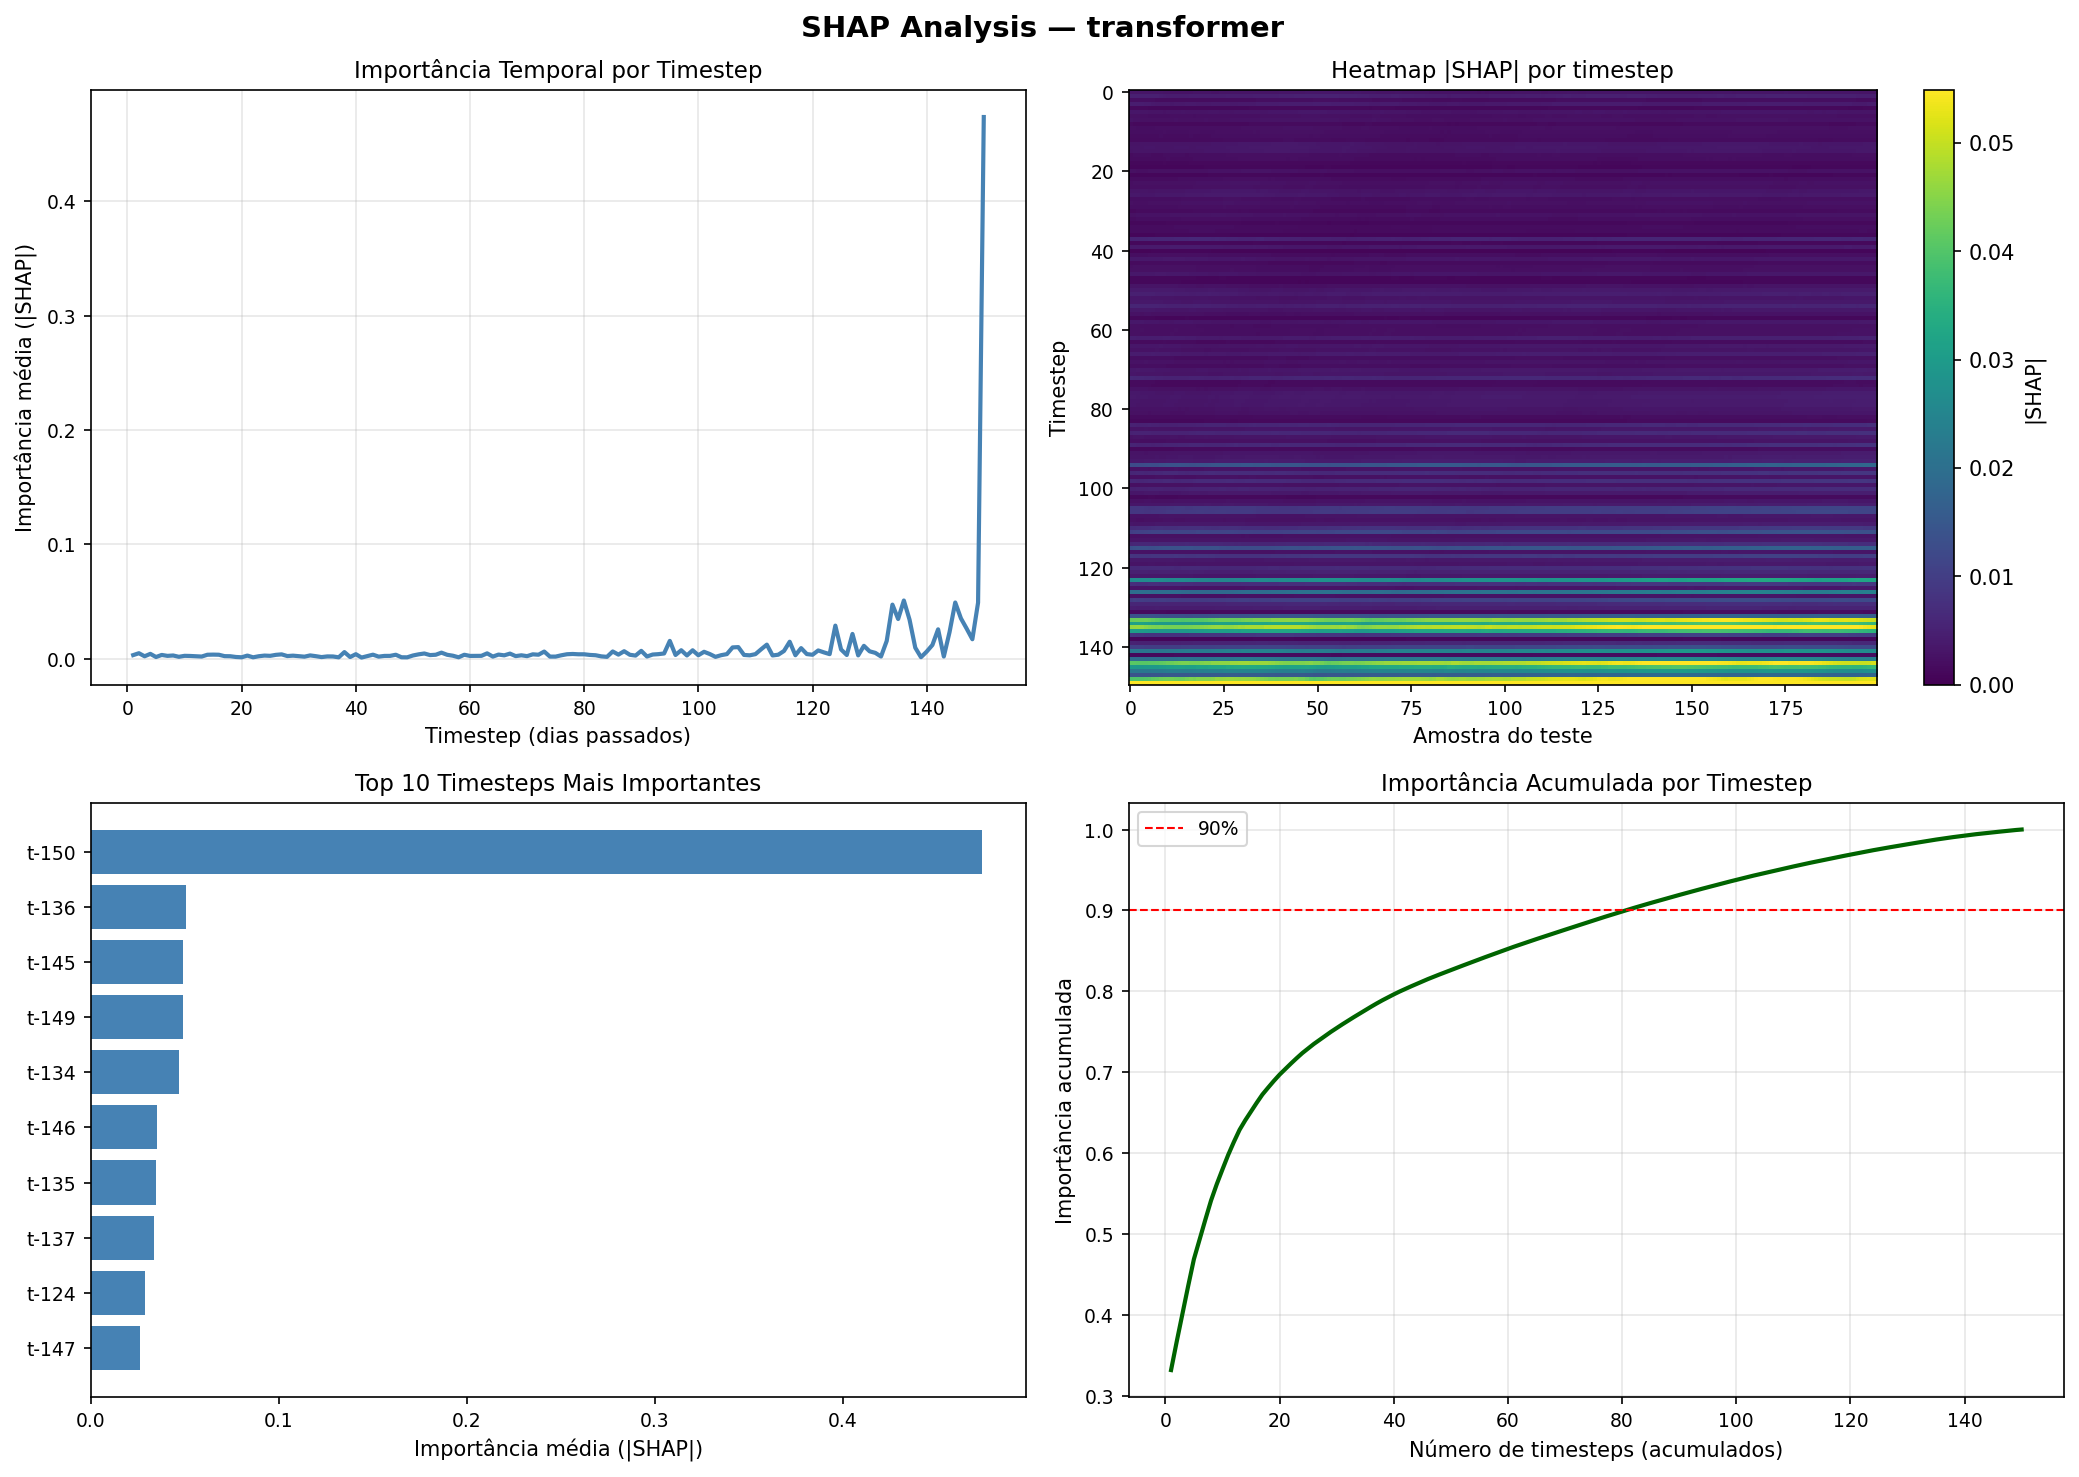
\includegraphics[width=0.85\textwidth]{figuras/shap_transformer.png}
    \caption{Análise SHAP do Transformer-TS no conjunto de teste (2023--2024)}
\end{figure}
\end{frame}


\begin{frame}{Principais Resultados}
\begin{enumerate}
    \item \textbf{\textit{DWT} é o pré-processamento mais impactante:} variantes com \textit{DWT} superam consistentemente as sem \textit{DWT} em \textit{MCC}
    \item \textbf{Sinal direcional consistente:} modelos \textit{SOTA} obtiveram 75--76\% de acurácia, contrastando com $R^2$ divergente
    \item \textbf{Limitação do \textit{Min-Max}:} saturação ao prever preços acima do máximo do treino (3.756 USD vs. 5.000--6.000 USD em 2023--2024)
    \item \textbf{Janelas subutilizadas:} SHAP revela que modelos dependem predominantemente de curto prazo
\end{enumerate}
\end{frame}

%-------------------------------------------------------
\section{Conclusão}
%-------------------------------------------------------

\begin{frame}{Conclusão}
\begin{itemize}
    \item Variante B (\textit{DWT} + \textit{Z-score}) obteve melhor desempenho no \textit{ablation study}
    \item Modelos \textit{SOTA} superaram LSTM em acurácia direcional (+8 pontos percentuais)
    \item SHAP revelou concentração de atenção no passado imediato
    \item Janela de 150 dias não foi totalmente utilizada, indicando que as arquiteturas SOTA conseguem previsões mais corretas mesmo com contexto histórico
\end{itemize}
\end{frame}

\begin{frame}{Conclusão}
\textbf{Limitações:}
\begin{itemize}
    \item Saturação da normalização \textit{Min-Max}
    \item Janela de entrada fixa
    \item Escopo univariado dos modelos \textit{SOTA}
    \item Dados de um único ativo e período
    \item Ausência de avaliação financeira
    \item Treino em regressão nos modelos \textit{SOTA}
\end{itemize}
\end{frame}

\begin{frame}{Conclusão}
\textbf{Trabalhos futuros:}
\begin{itemize}
    \item Modelos \textit{SOTA} focados em classificação direcional com pré processamento e \textit{inputs} validados do \textit{Ablation Study}
    \item Avaliação de retorno financeiro
    \item Extensão para IBOVESPA
\end{itemize}
\end{frame}

% %-------------------------------------------------------
% \section{Cronograma}
% %-------------------------------------------------------

% \begin{frame}{Cronograma de Atividades}
% \begin{table}[H]
% \centering
% \resizebox{\textwidth}{!}{%
% \begin{tabular}{|l|c|c|c|c|c|c|c|c|c|c|c|c|c|c|c|c|}
% \hline
% \textbf{Atividade} & \textbf{S1} & \textbf{S2} & \textbf{S3} & \textbf{S4} & \textbf{S5} & \textbf{S6} & \textbf{S7} & \textbf{S8} & \textbf{S9} & \textbf{S10} & \textbf{S11} & \textbf{S12} & \textbf{S13} & \textbf{S14} & \textbf{S15} & \textbf{S16} \\
% \hline
% Aquisição de Dados & $\bullet$ & $\bullet$ &  &  &  &  &  &  &  &  &  &  &  &  &  &  \\
% \hline
% Pré-processamento &  & $\bullet$ & $\bullet$ & $\bullet$ &  &  &  &  &  &  &  &  &  &  &  &  \\
% \hline
% Modelagem &  &  &  & $\bullet$ & $\bullet$ & $\bullet$ &  &  &  &  &  &  &  &  &  &  \\
% \hline
% Treinamento &  &  &  &  &  & $\bullet$ & $\bullet$ & $\bullet$ &  &  &  &  &  &  &  &  \\
% \hline
% Avaliação e Validação &  &  &  &  &  &  &  & $\bullet$ & $\bullet$ & $\bullet$ & $\bullet$ & $\bullet$ &  &  &  &  \\
% \hline
% Interpretabilidade (xAI) &  &  &  &  &  &  &  &  &  &  & $\bullet$ & $\bullet$ & $\bullet$ & $\bullet$ &  &  \\
% \hline
% Escrita do Relatório &  &  &  &  & $\bullet$ & $\bullet$ & $\bullet$ & $\bullet$ & $\bullet$ & $\bullet$ & $\bullet$ & $\bullet$ & $\bullet$ & $\bullet$ &  &  \\
% \hline
% Revisão e Ajustes &  &  &  &  &  &  &  &  &  &  &  &  &  & $\bullet$ & $\bullet$ & $\bullet$ \\
% \hline
% \end{tabular}%
% }
% \end{table}
% \end{frame}

%-------------------------------------------------------
% \begin{frame}{Considerações Finais}
% \begin{itemize}
%     \item LSTM captura dependências temporais do IBOVESPA; xAI (SHAP) traz transparência para as previsões.
%     \item Resultados esperados: erro reduzido (RMSE, $R^2$ competitivo) e entendimento das \textit{features} mais influentes.
%     \item Próximos passos: refinar hiperparâmetros, avaliar rentabilidade financeira e consolidar visualizações para defesa.
% \end{itemize}
% \end{frame}

%-------------------------------------------------------
\begin{frame}[plain,noframenumbering]
  \finalpage{\Large{Obrigado pela atenção.}}
\end{frame}


\end{document}